%Uebung 1
\setcounter{section}{1}
\setcounter{subsection}{0}
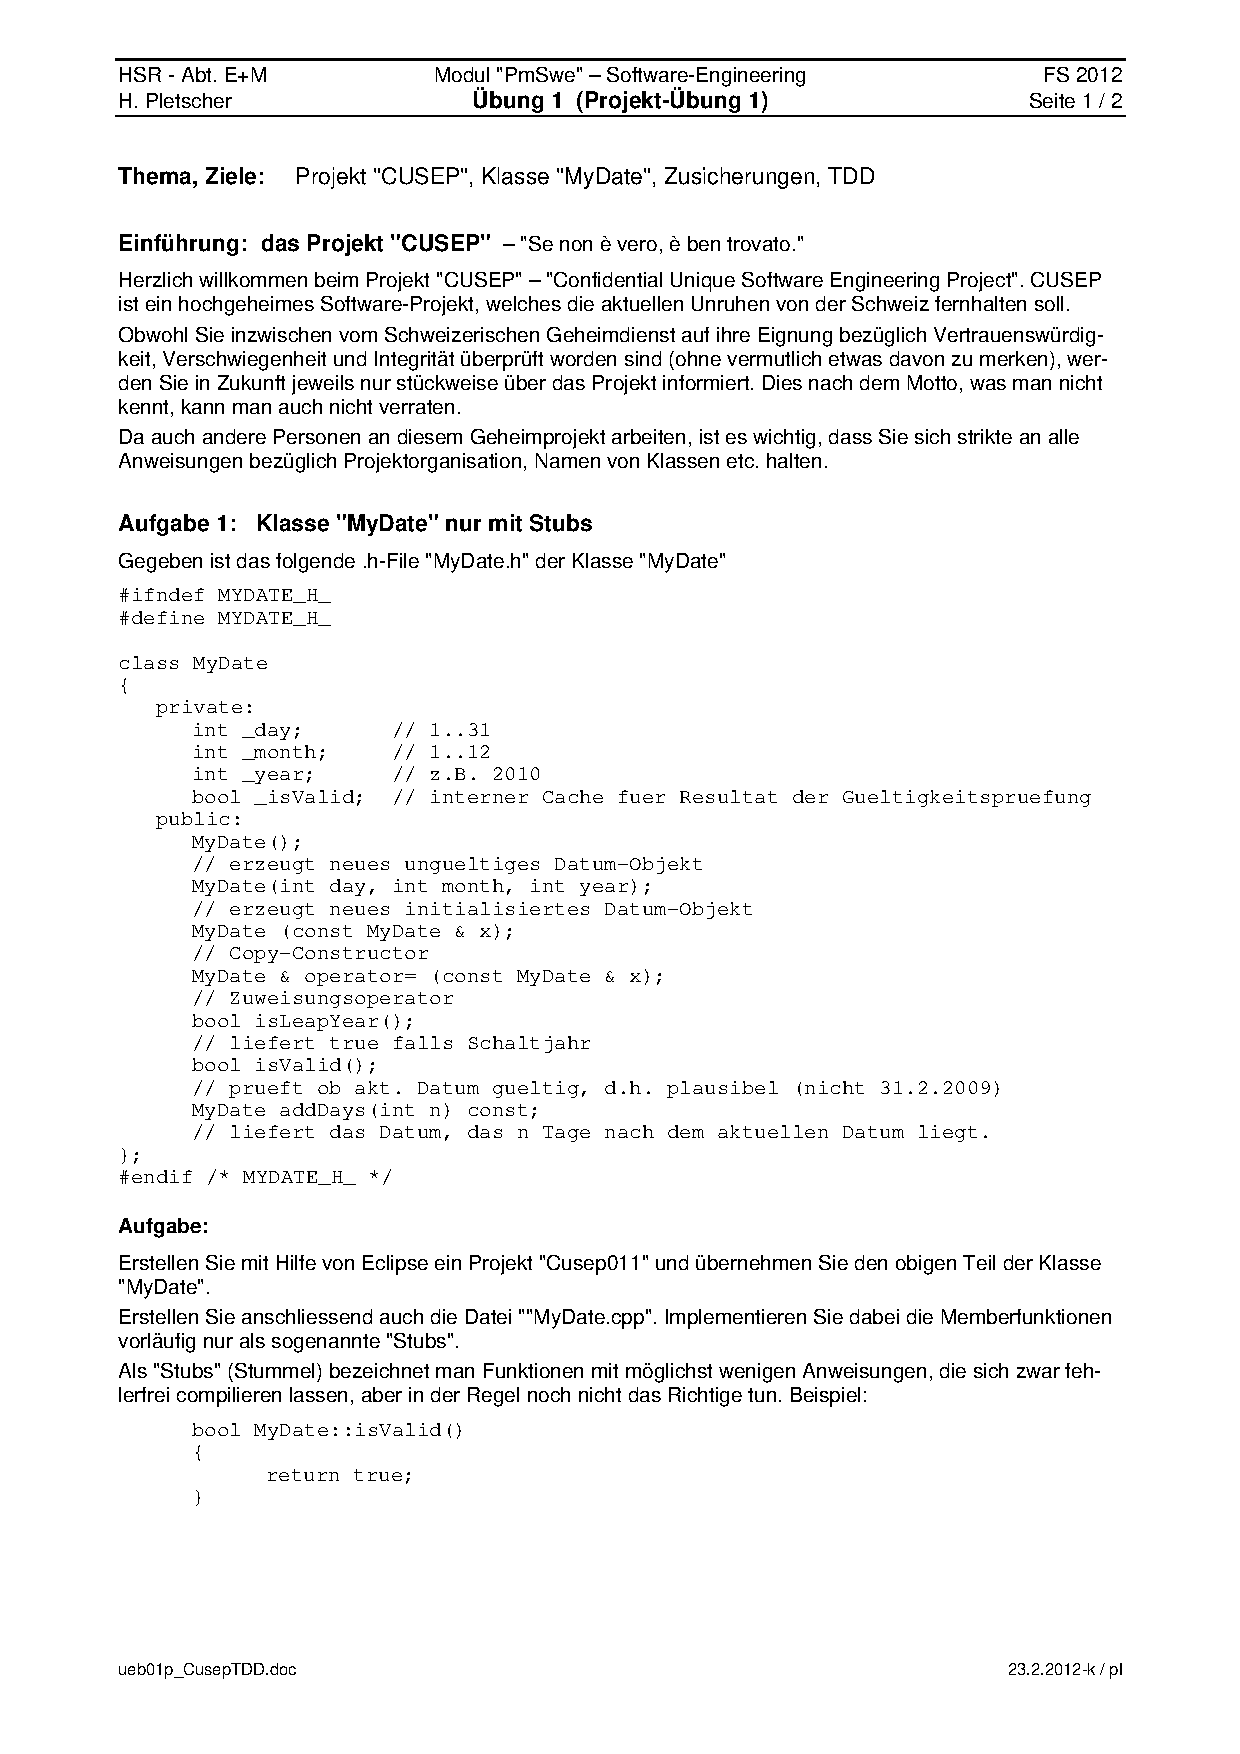
\includepdf[pages=-]{./UebAufgaben/ueb01p_CusepTDD.pdf}
\subsection{Lösung}
\subsubsection{MyDate.h}
\lstinputlisting{./UebLoesungen/LoesUeb01_Cusep1/MyDate.h}
\subsubsection{MyDate.cpp}
\lstinputlisting{./UebLoesungen/LoesUeb01_Cusep1/MyDate.cpp}
\subsubsection{testMyDate.cpp}
\lstinputlisting{./UebLoesungen/LoesUeb01_Cusep1/testMyDate.cpp}

%Uebung 2
\setcounter{section}{2}
\setcounter{subsection}{1}
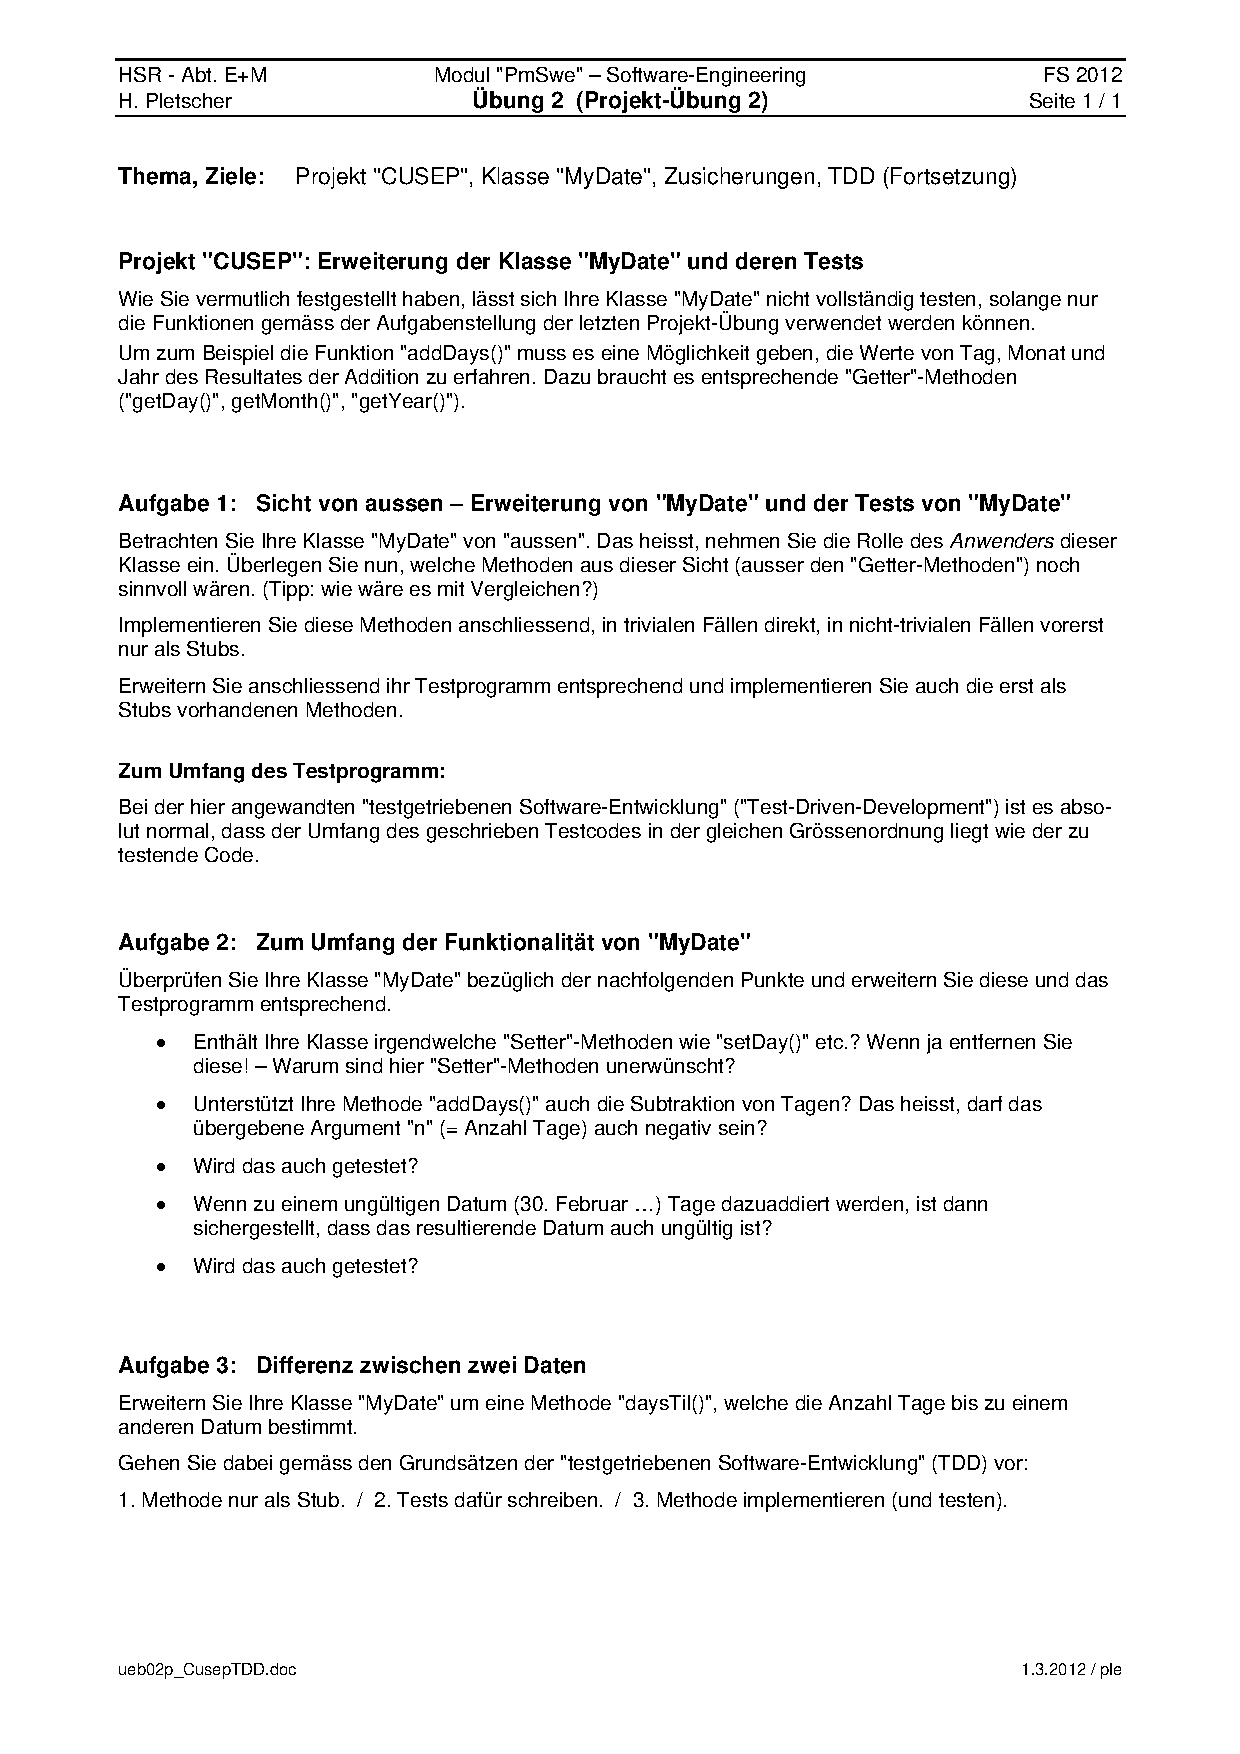
\includepdf[pages=-]{./UebAufgaben/ueb02p_CusepTDD.pdf}
\subsection{Lösung}
\subsubsection{MyDate.h}
\lstinputlisting{./UebLoesungen/LoesUeb02_Cusep2/MyDate.h}
\subsubsection{MyDate.cpp}
\lstinputlisting{./UebLoesungen/LoesUeb02_Cusep2/MyDate.cpp}
\subsubsection{testMyDate.cpp}
\lstinputlisting{./UebLoesungen/LoesUeb02_Cusep2/testMyDate.cpp}

%Uebung 3
\setcounter{section}{3}
\setcounter{subsection}{1}
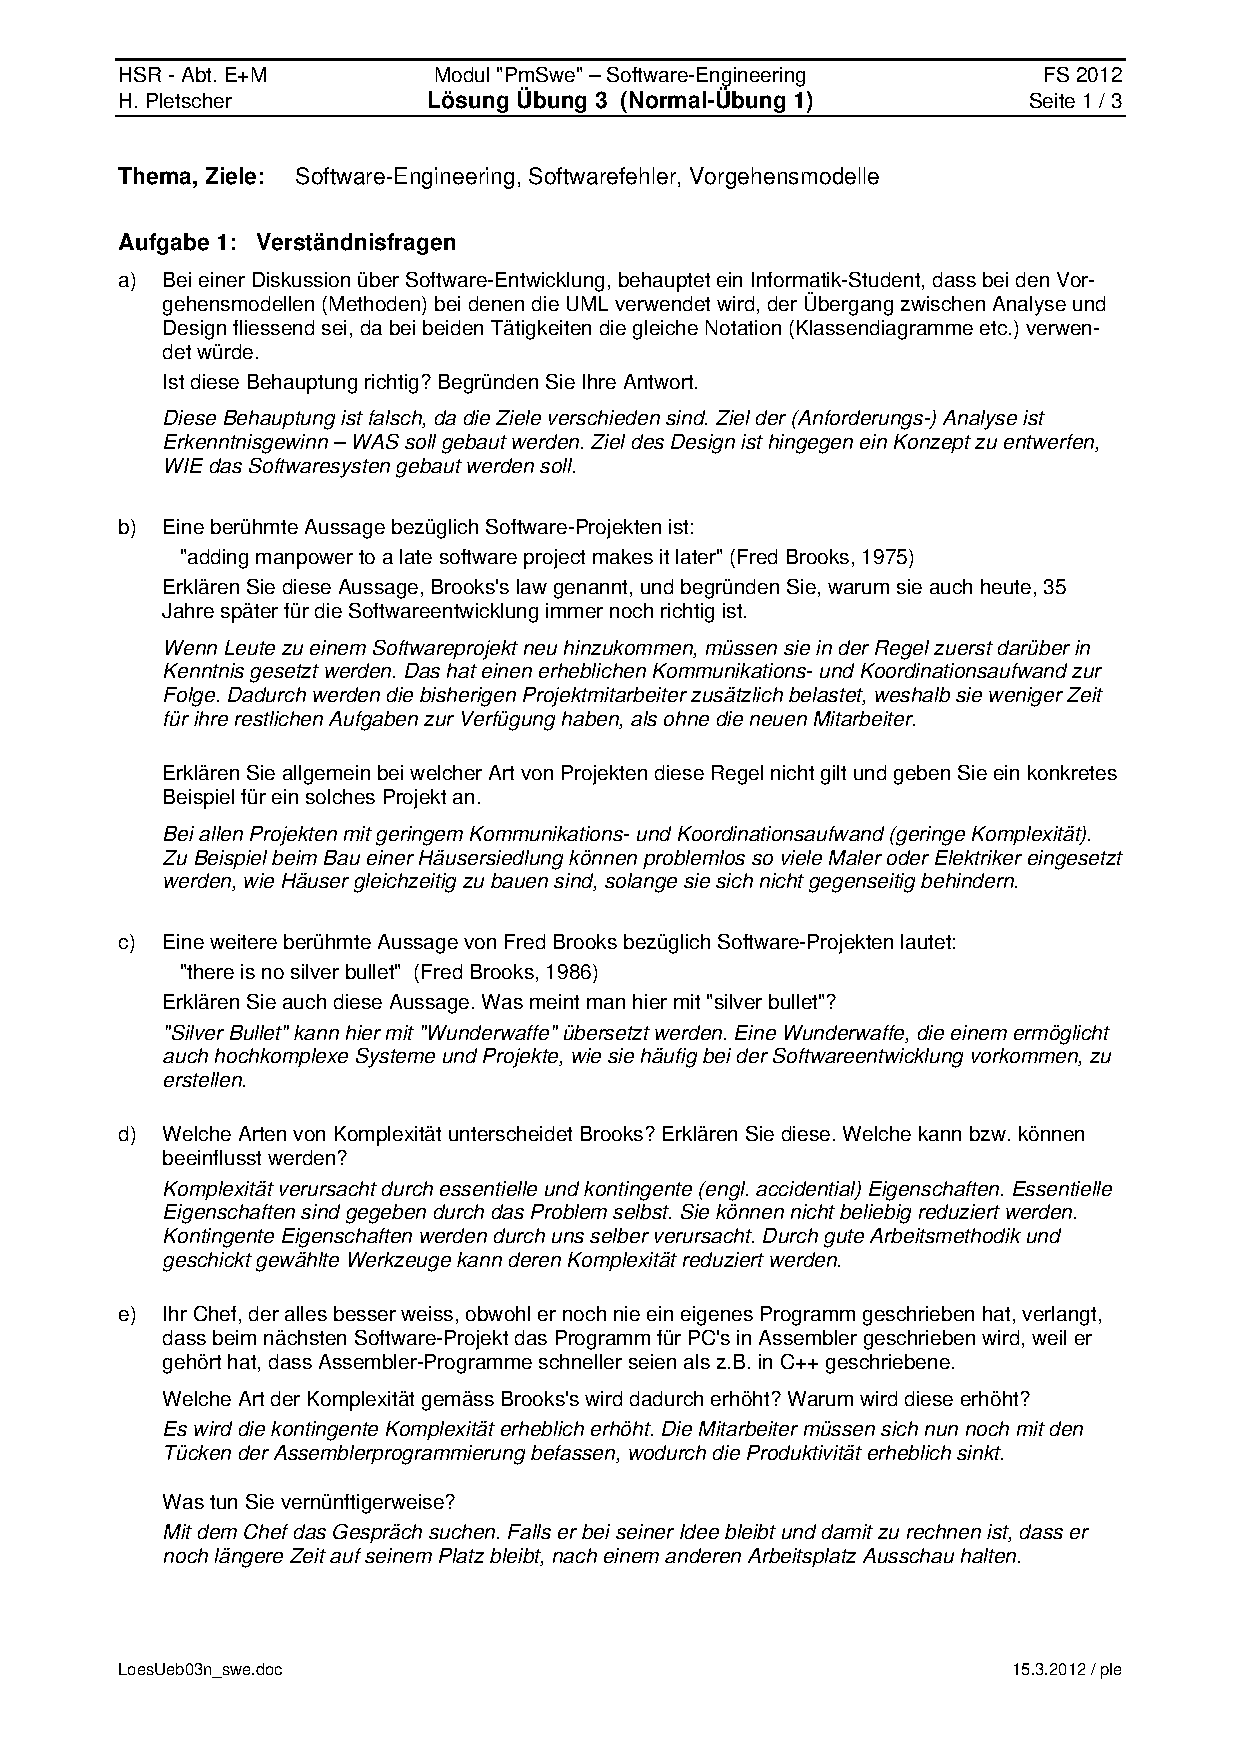
\includepdf[pages=-]{./UebLoesungen/LoesUeb03_swe/LoesUeb03n_swe.pdf}

%Uebung 4
\setcounter{section}{4}
\setcounter{subsection}{1}
\setcounter{subsubsection}{1}
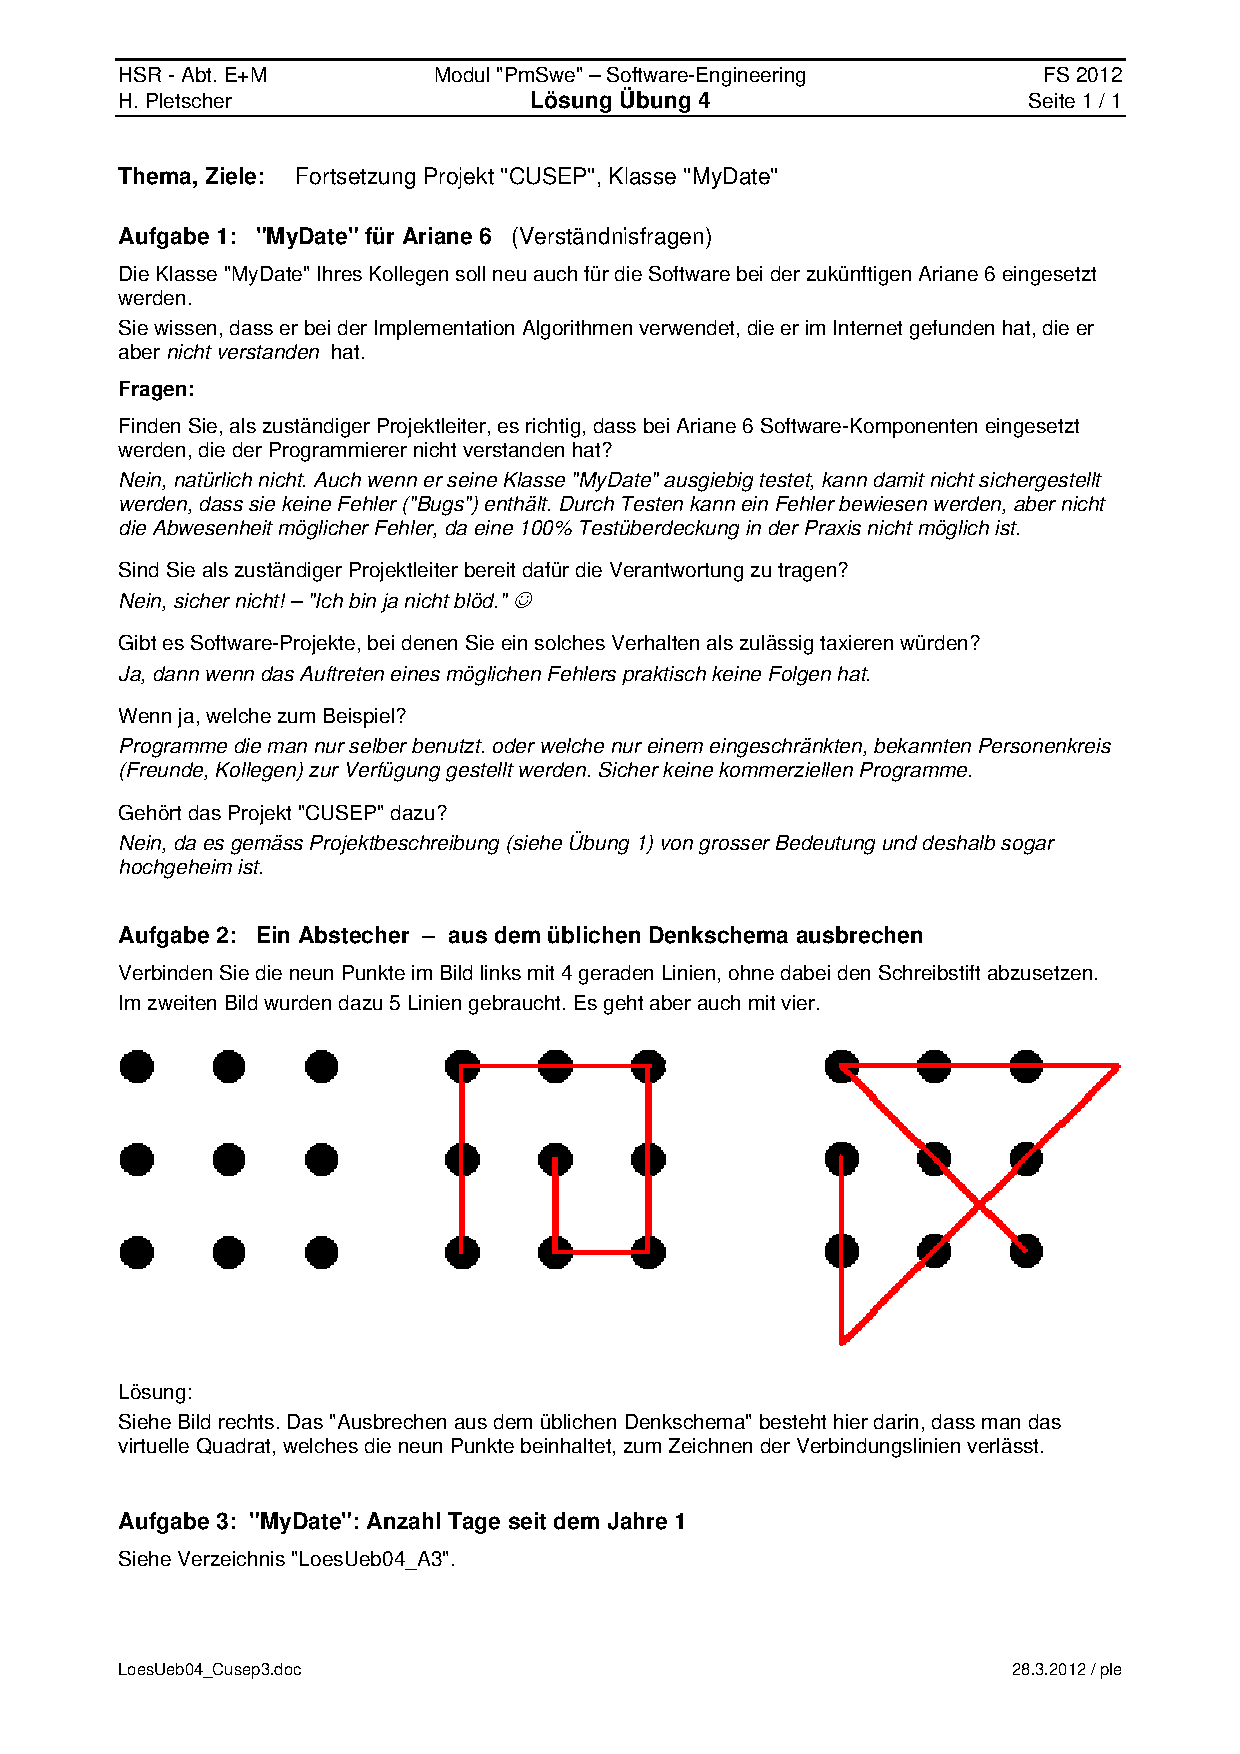
\includepdf[pages=-]{./UebLoesungen/LoesUeb04_Cusep3/LoesUeb04_Cusep3.pdf}
\subsection{Lösung}
\subsubsection{MyDate.h}
\lstinputlisting{./UebLoesungen/LoesUeb04_Cusep3/LoesUeb04_A3_MyDate/MyDate.h}
\subsubsection{MyDate.cpp}
\lstinputlisting{./UebLoesungen/LoesUeb04_Cusep3/LoesUeb04_A3_MyDate/MyDate.cpp}
\subsubsection{testMyDate.cpp}
\lstinputlisting{./UebLoesungen/LoesUeb04_Cusep3/LoesUeb04_A3_MyDate/testMyDate.cpp}

%Uebung 5
\setcounter{section}{5}
\setcounter{subsection}{1}
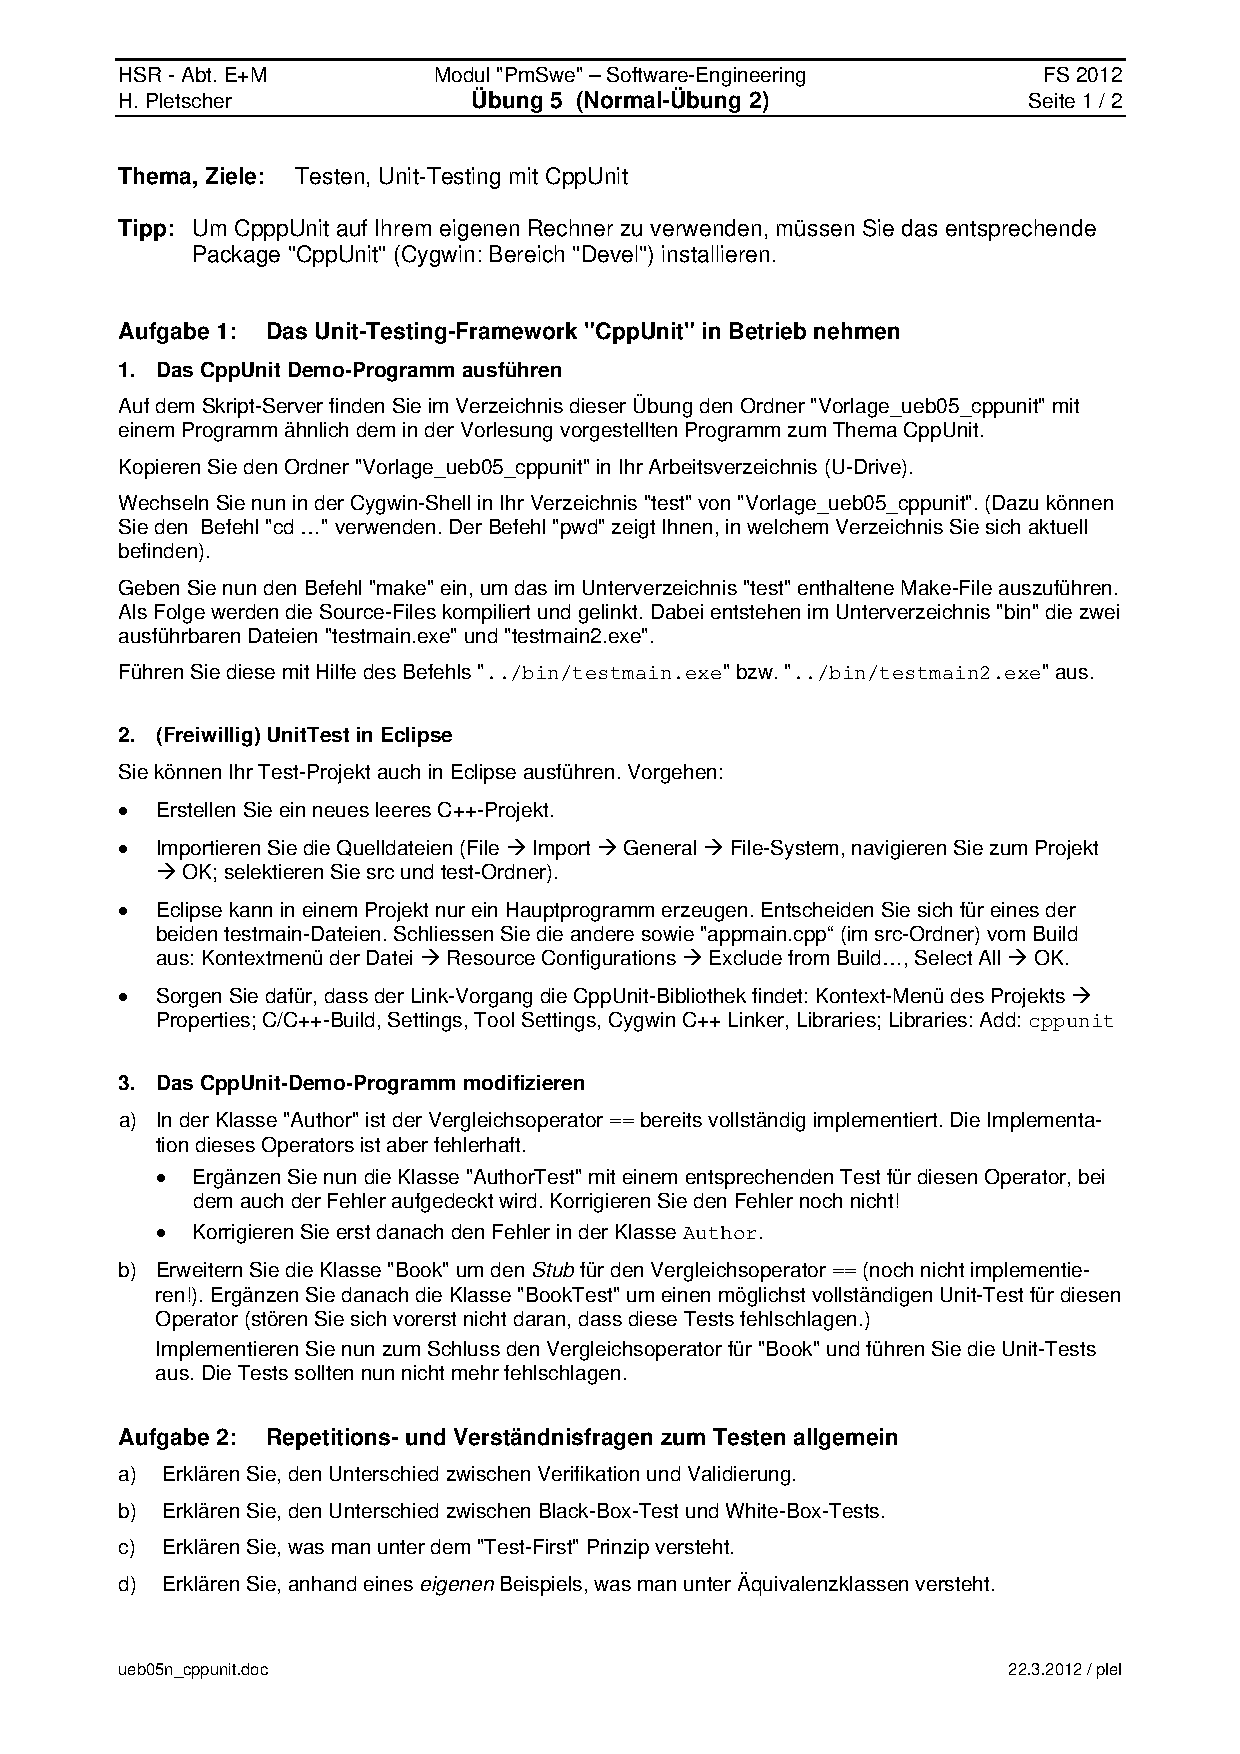
\includepdf[pages=-]{./UebAufgaben/ueb05n_cppunit.pdf}
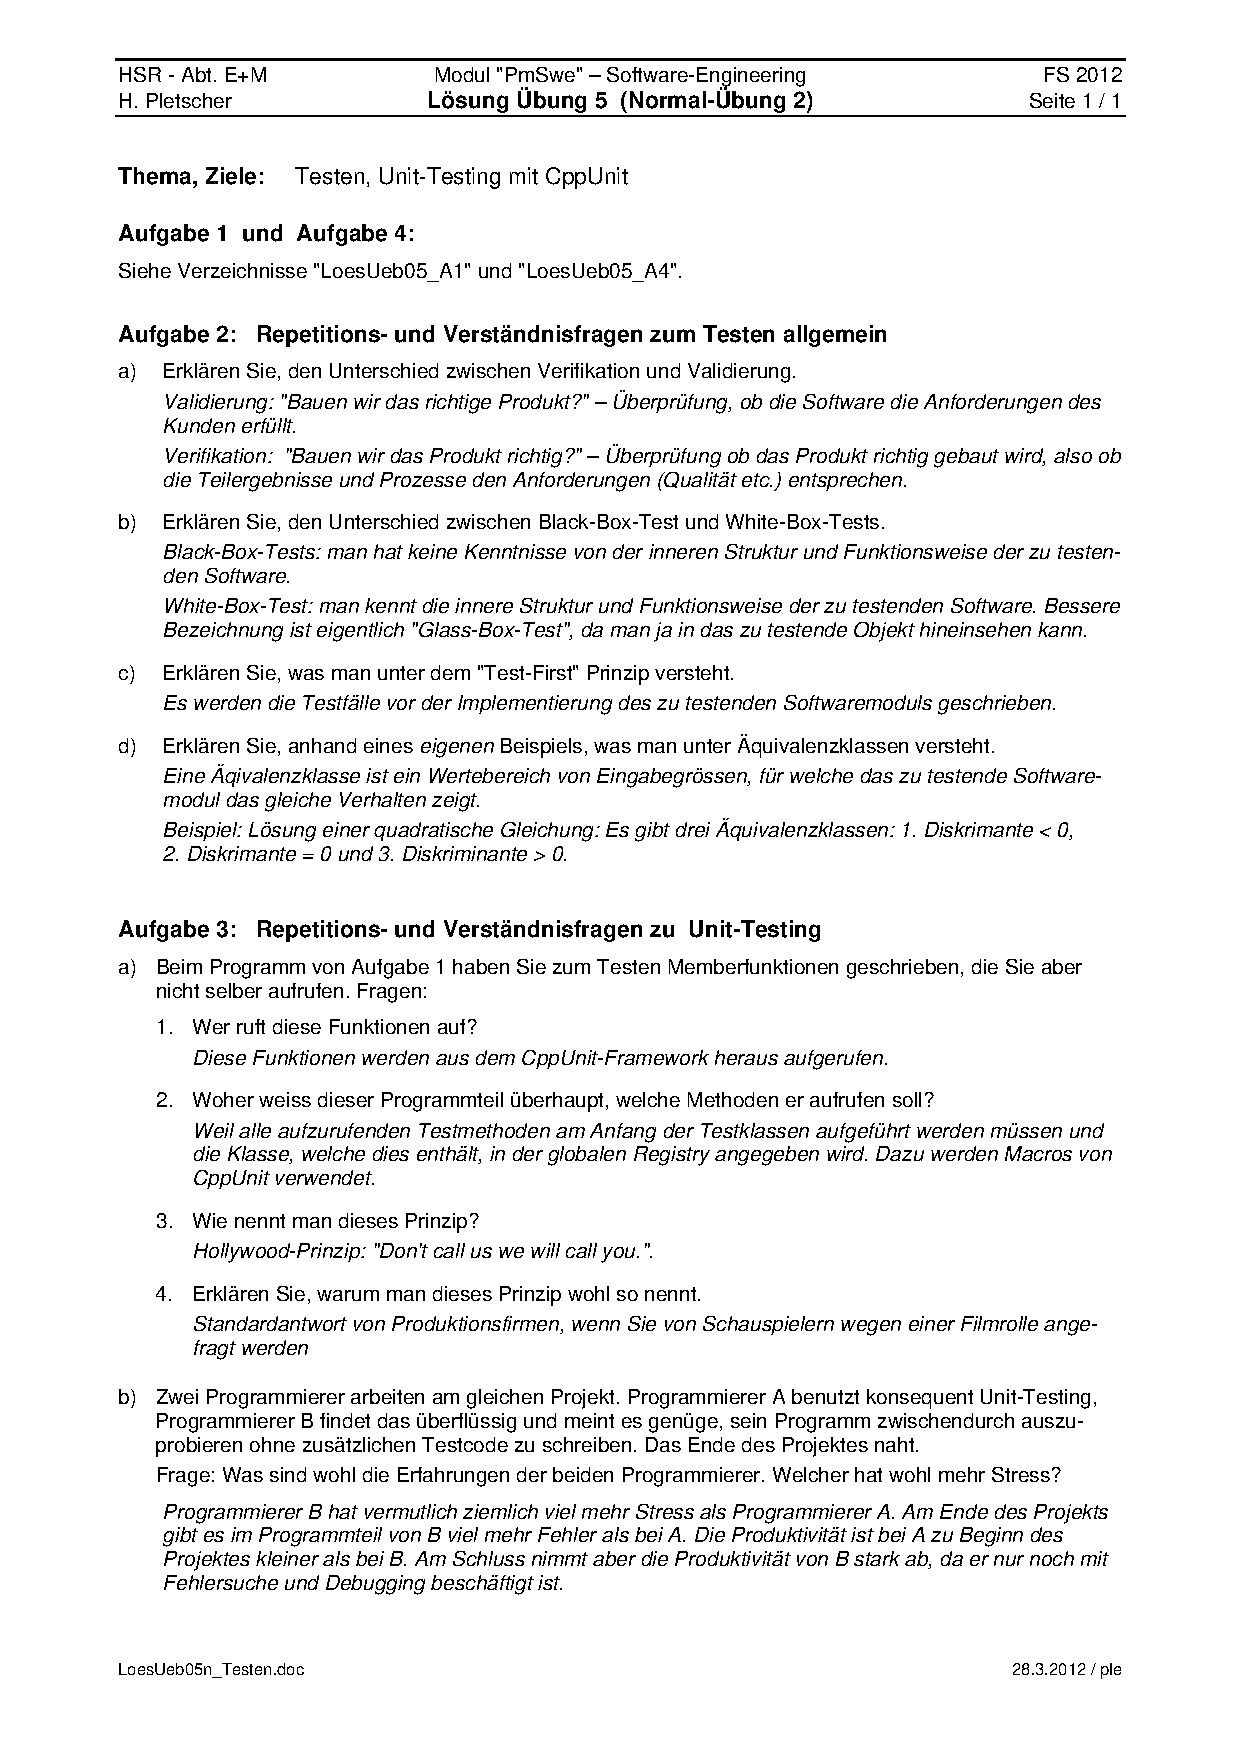
\includepdf[pages=-]{./UebLoesungen/LoesUeb05_testen/LoesUeb05n_Testen.pdf}
\subsection{Lösung Aufgabe 1}
\subsubsection{appmain.cpp}
\lstinputlisting{./UebLoesungen/LoesUeb05_testen/LoesUeb05_A1_cppunit/src/appmain.cpp}
\subsubsection{Author.cpp}
\lstinputlisting{./UebLoesungen/LoesUeb05_testen/LoesUeb05_A1_cppunit/src/Author.cpp}
\subsubsection{Author.h}
\lstinputlisting{./UebLoesungen/LoesUeb05_testen/LoesUeb05_A1_cppunit/src/Author.h}
\subsubsection{Book.cpp}
\lstinputlisting{./UebLoesungen/LoesUeb05_testen/LoesUeb05_A1_cppunit/src/Book.cpp}
\subsubsection{Book.h}
\lstinputlisting{./UebLoesungen/LoesUeb05_testen/LoesUeb05_A1_cppunit/src/Book.h}
\subsubsection{MyTools.cpp}
\lstinputlisting{./UebLoesungen/LoesUeb05_testen/LoesUeb05_A1_cppunit/src/MyTools.cpp}
\subsubsection{MyTools.h}
\lstinputlisting{./UebLoesungen/LoesUeb05_testen/LoesUeb05_A1_cppunit/src/MyTools.h}

\subsection{Lösung Aufgabe 4}
\setcounter{subsection}{1}
\subsubsection{MyDate.cpp}
\lstinputlisting{./UebLoesungen/LoesUeb05_testen/LoesUeb05_A4_mydate/src/MyDate.cpp}
\subsubsection{MyDate.h}
\lstinputlisting{./UebLoesungen/LoesUeb05_testen/LoesUeb05_A4_mydate/src/MyDate.h}
\subsubsection{MyDate\_\_.cpp}
\lstinputlisting{./UebLoesungen/LoesUeb05_testen/LoesUeb05_A4_mydate/src/MyDate__.cpp}
\subsubsection{MyDate\_\_.h}
\lstinputlisting{./UebLoesungen/LoesUeb05_testen/LoesUeb05_A4_mydate/src/MyDate__.h}

%Uebung 6
\setcounter{section}{6}
\setcounter{subsection}{1}
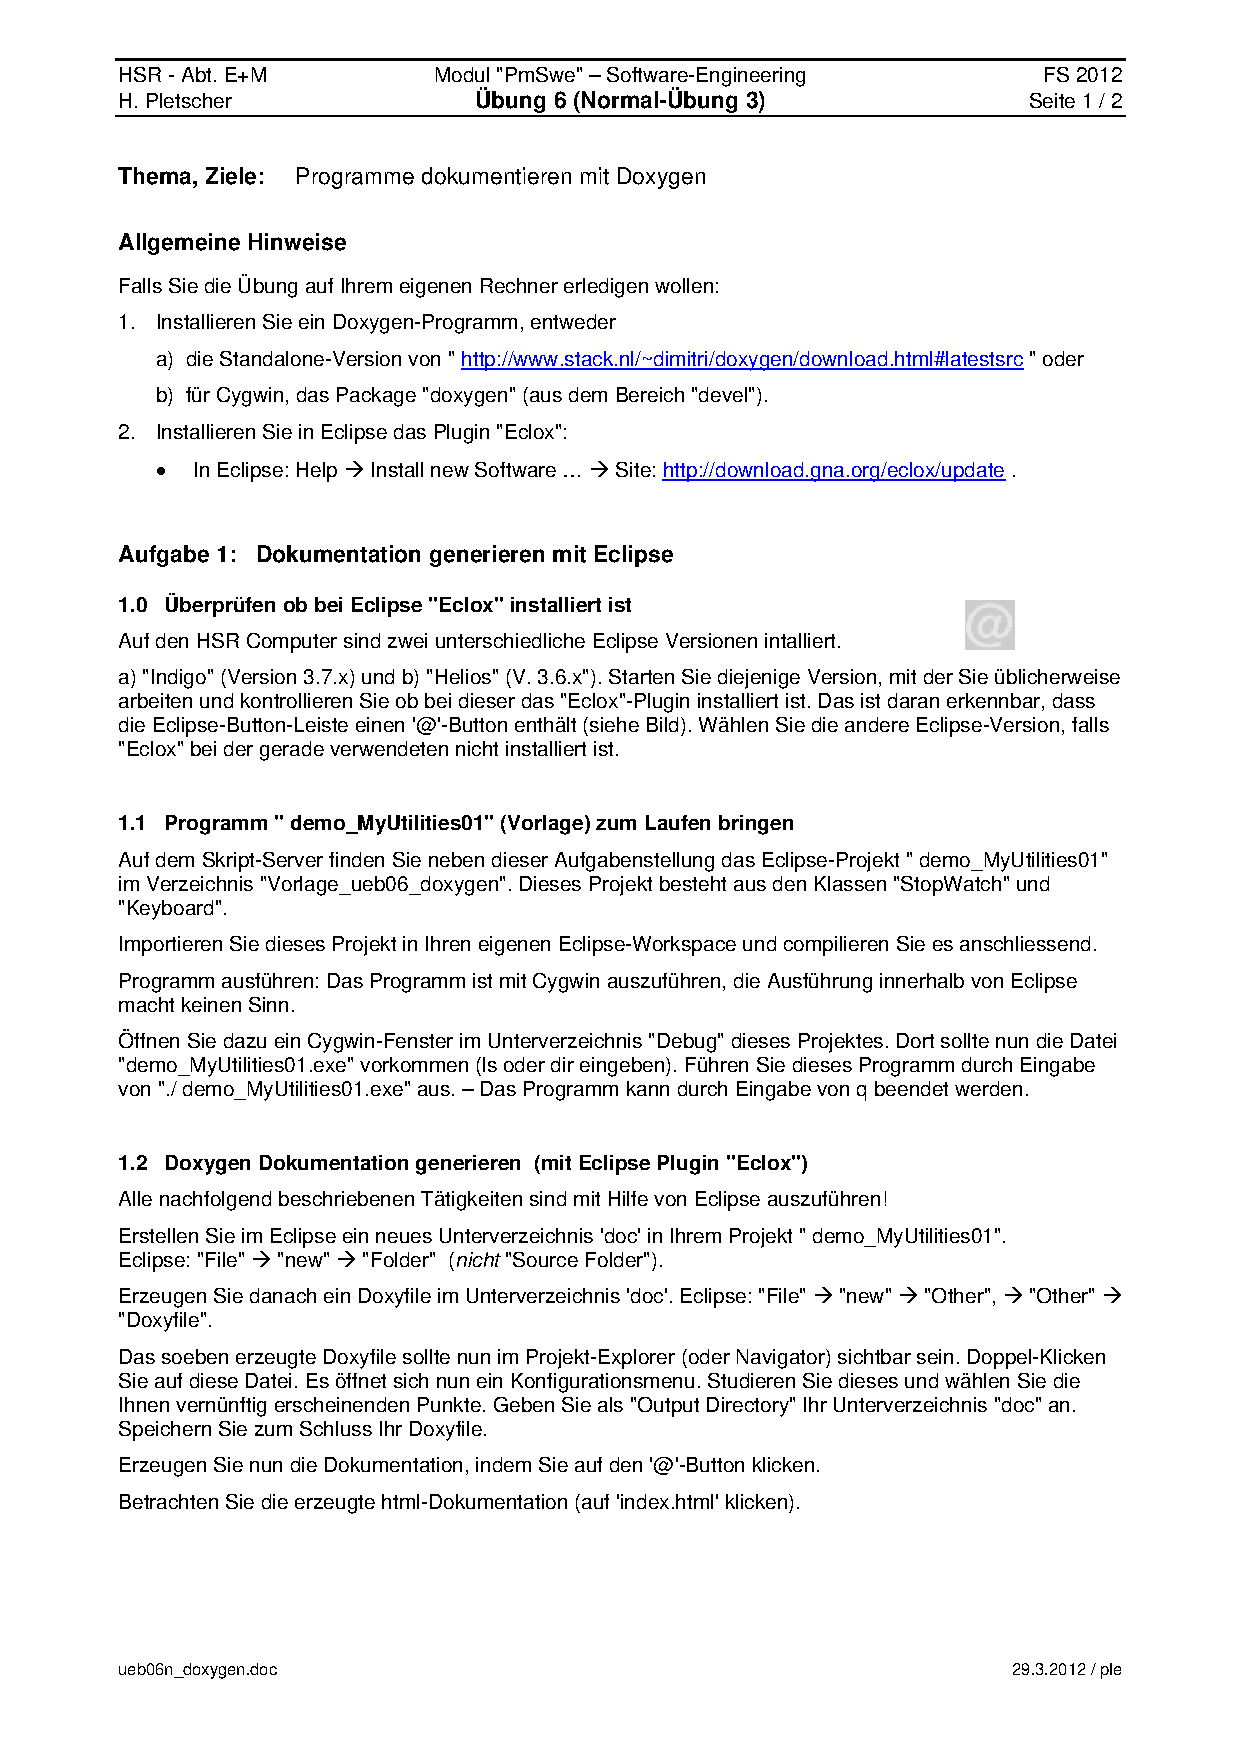
\includepdf[pages=-]{./UebAufgaben/ueb06n_doxygen.pdf}
\subsection{Lösung}
\subsubsection{demo\_MyUtilities01.cpp}
\lstinputlisting{./UebLoesungen/LoesUeb06_doxygen/demo_MyUtilities01.cpp}
\subsubsection{Keyboard.cpp}
\lstinputlisting{./UebLoesungen/LoesUeb06_doxygen/Keyboard.cpp}
\subsubsection{Keyboard.h}
\lstinputlisting{./UebLoesungen/LoesUeb06_doxygen/Keyboard.h}
\subsubsection{mainpage.h}
\lstinputlisting{./UebLoesungen/LoesUeb06_doxygen/mainpage.h}
\subsubsection{StopWatch.cpp}
\lstinputlisting{./UebLoesungen/LoesUeb06_doxygen/StopWatch.cpp}
\subsubsection{StopWatch.h}
\lstinputlisting{./UebLoesungen/LoesUeb06_doxygen/StopWatch.h}

%Uebung 7
\setcounter{section}{7}
\setcounter{subsection}{1}
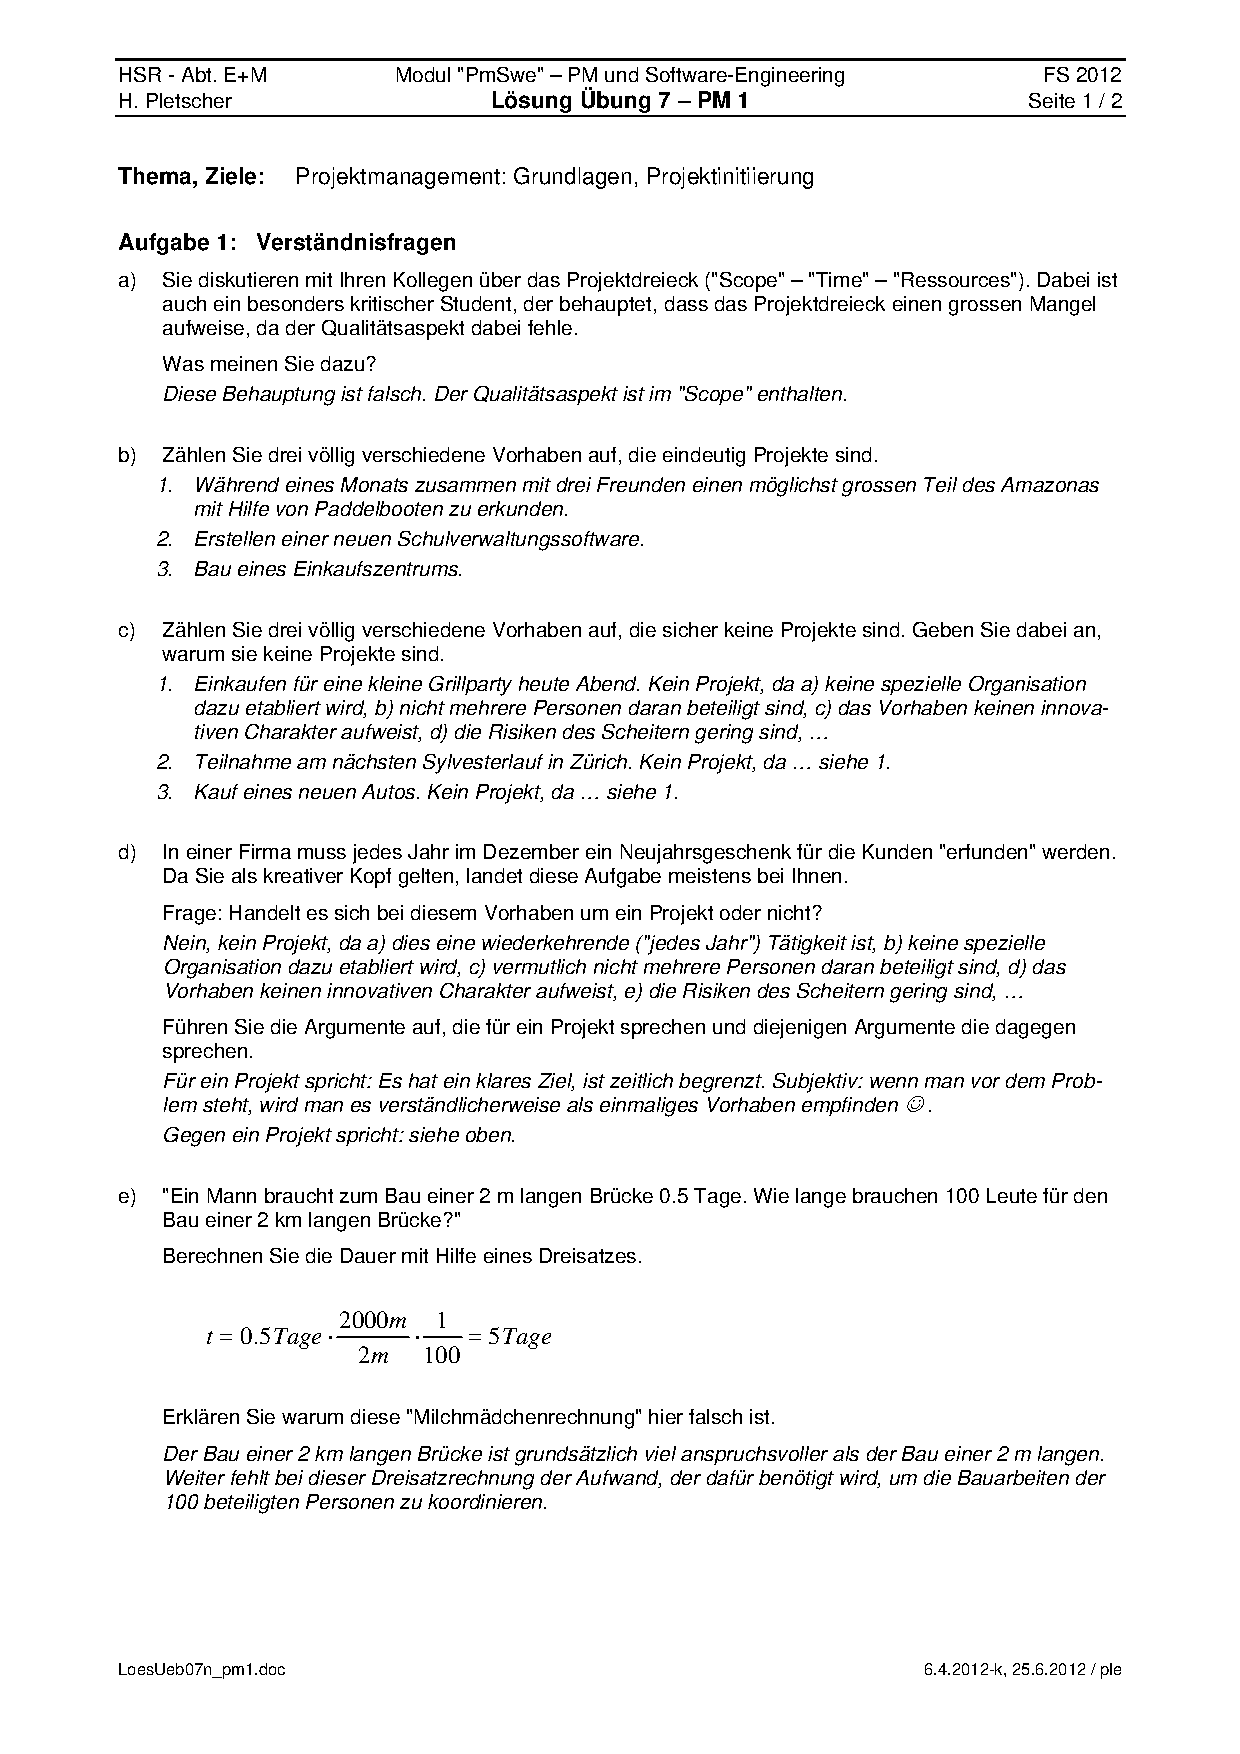
\includepdf[pages=-]{./UebLoesungen/LoesUeb07_pm1/LoesUeb07n_pm1.pdf}

%Uebung 8
\setcounter{section}{8}
\setcounter{subsection}{1}
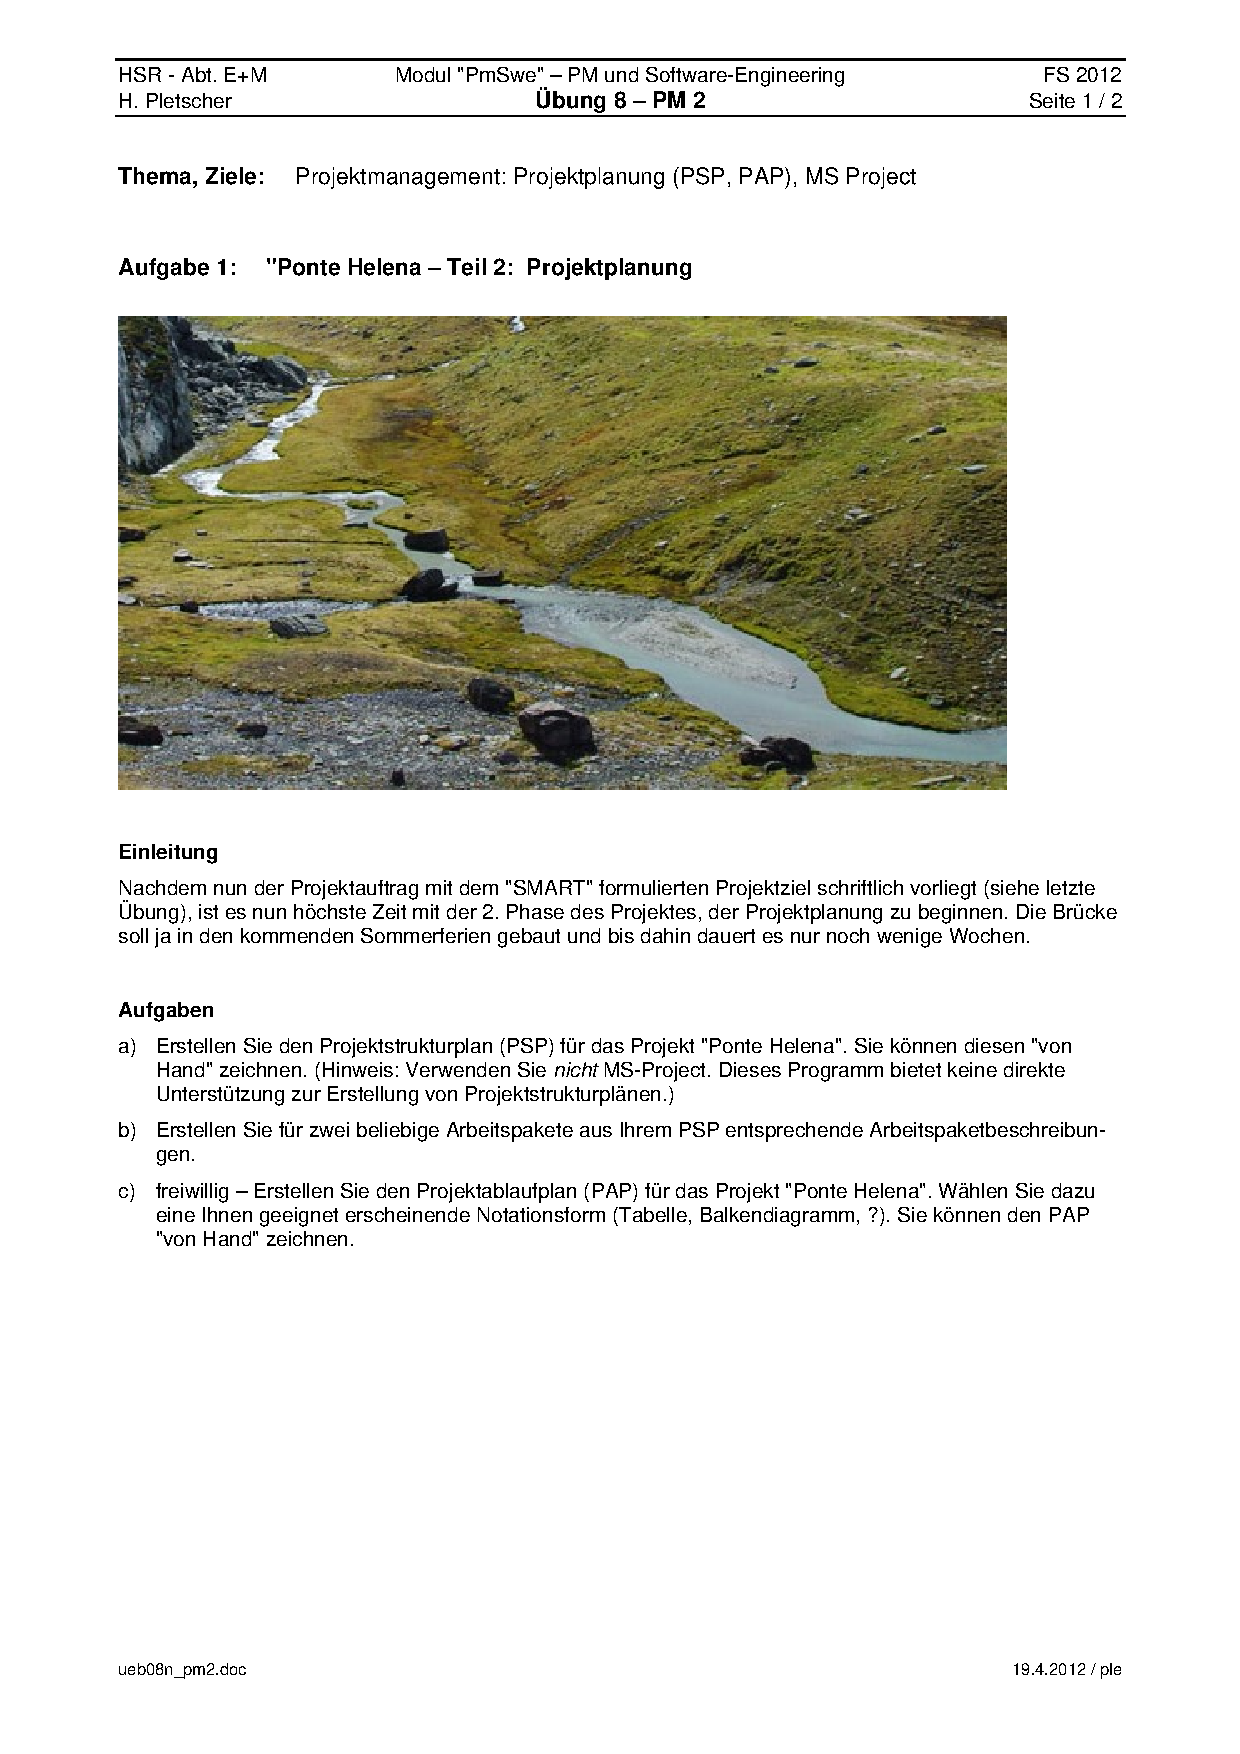
\includepdf[pages=-]{./UebAufgaben/ueb08n_pm2.pdf}
\subsection{Lösung}
\begin{center}
	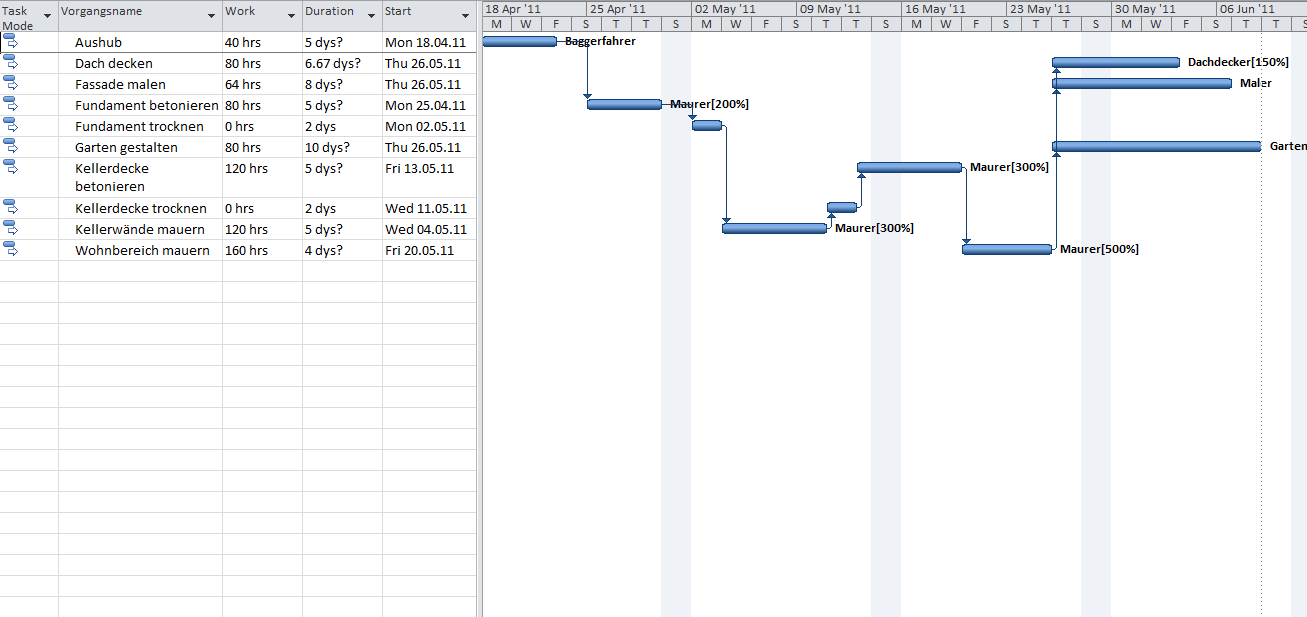
\includegraphics[angle=90,width=0.62\textwidth]{./UebLoesungen/LoesUeb08_pm2/ueb08_loesung.png}
\end{center}


%Uebung 9
\setcounter{section}{9}
\setcounter{subsection}{1}
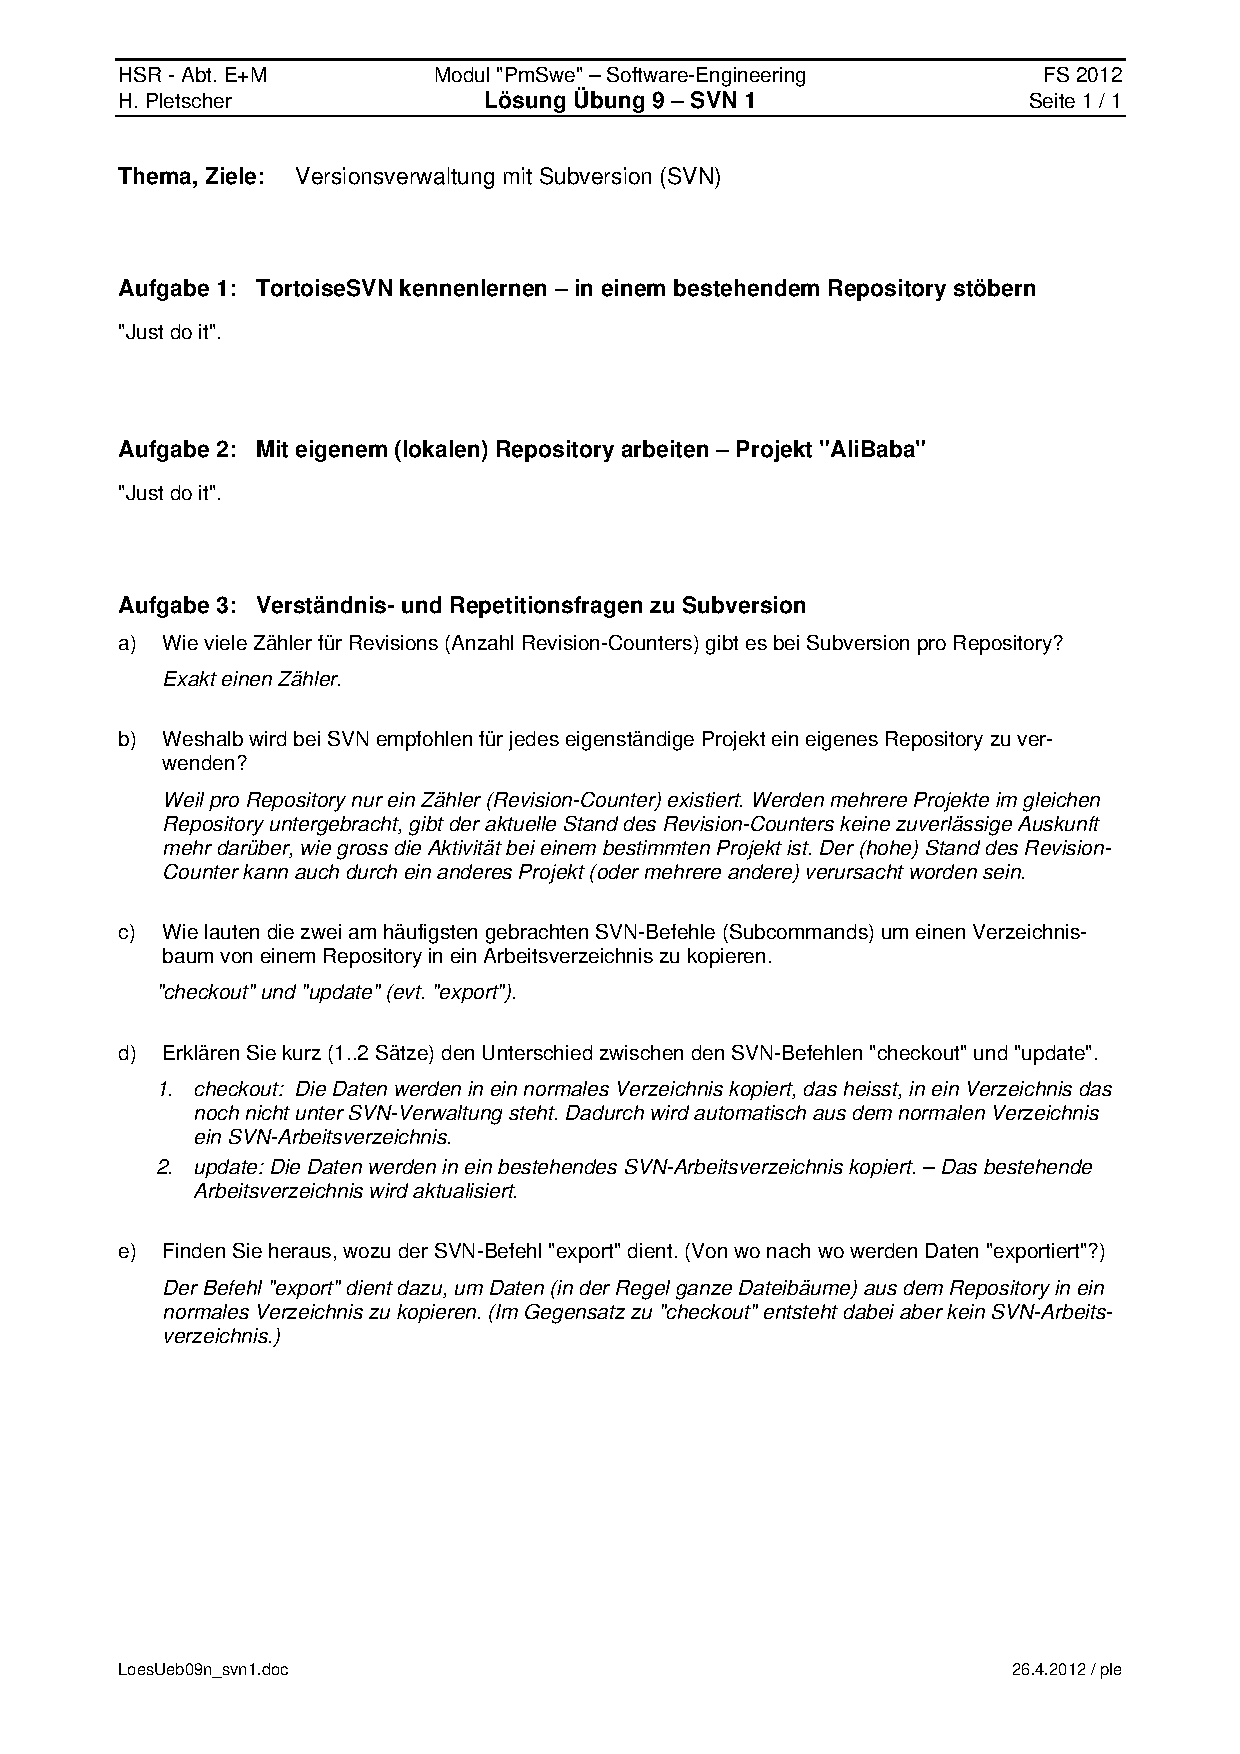
\includepdf[pages=-]{./UebLoesungen/LoesUeb09_svn1/LoesUeb09n_svn1.pdf}

%Uebung 10
\setcounter{section}{10}
\setcounter{subsection}{1}
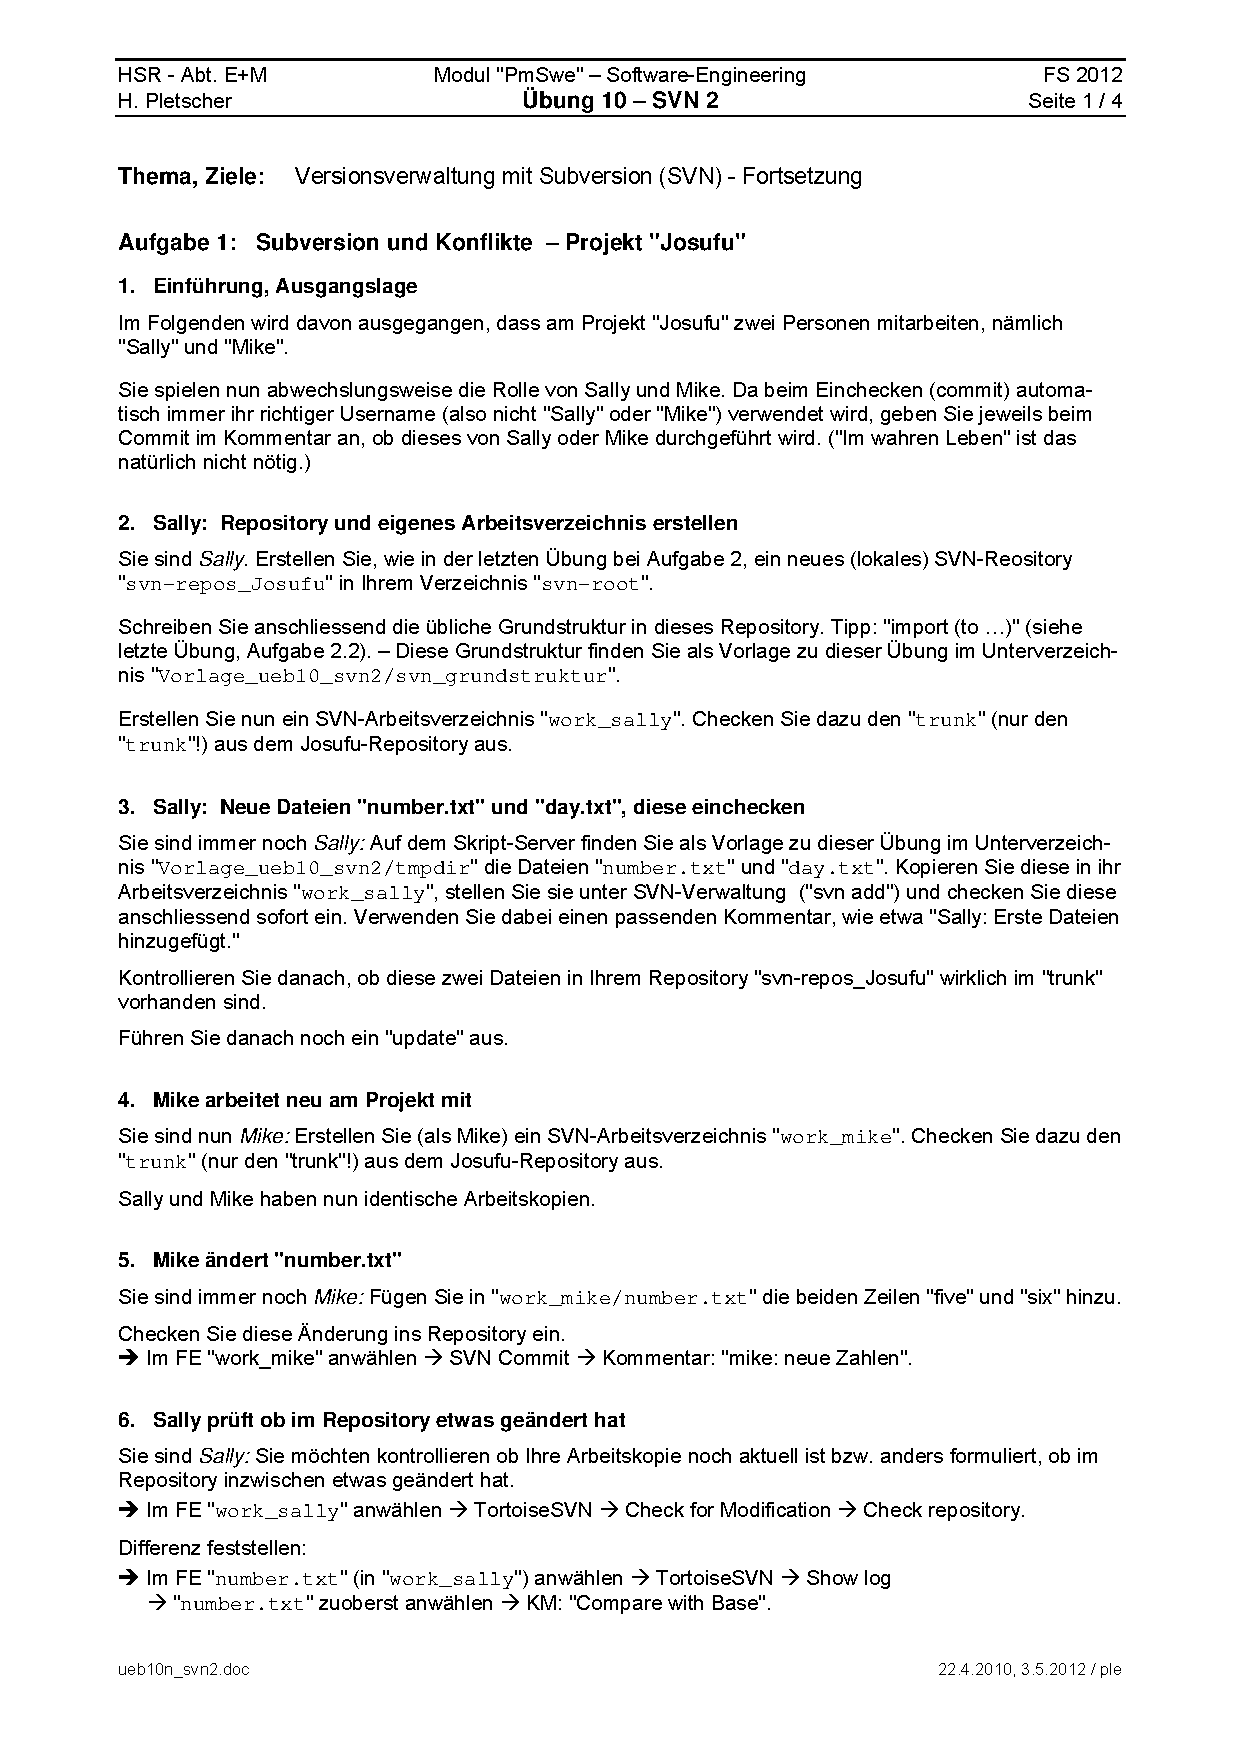
\includepdf[pages=-]{./UebAufgaben/ueb10n_svn2.pdf}

%Uebung 11
\setcounter{section}{11}
\setcounter{subsection}{1}
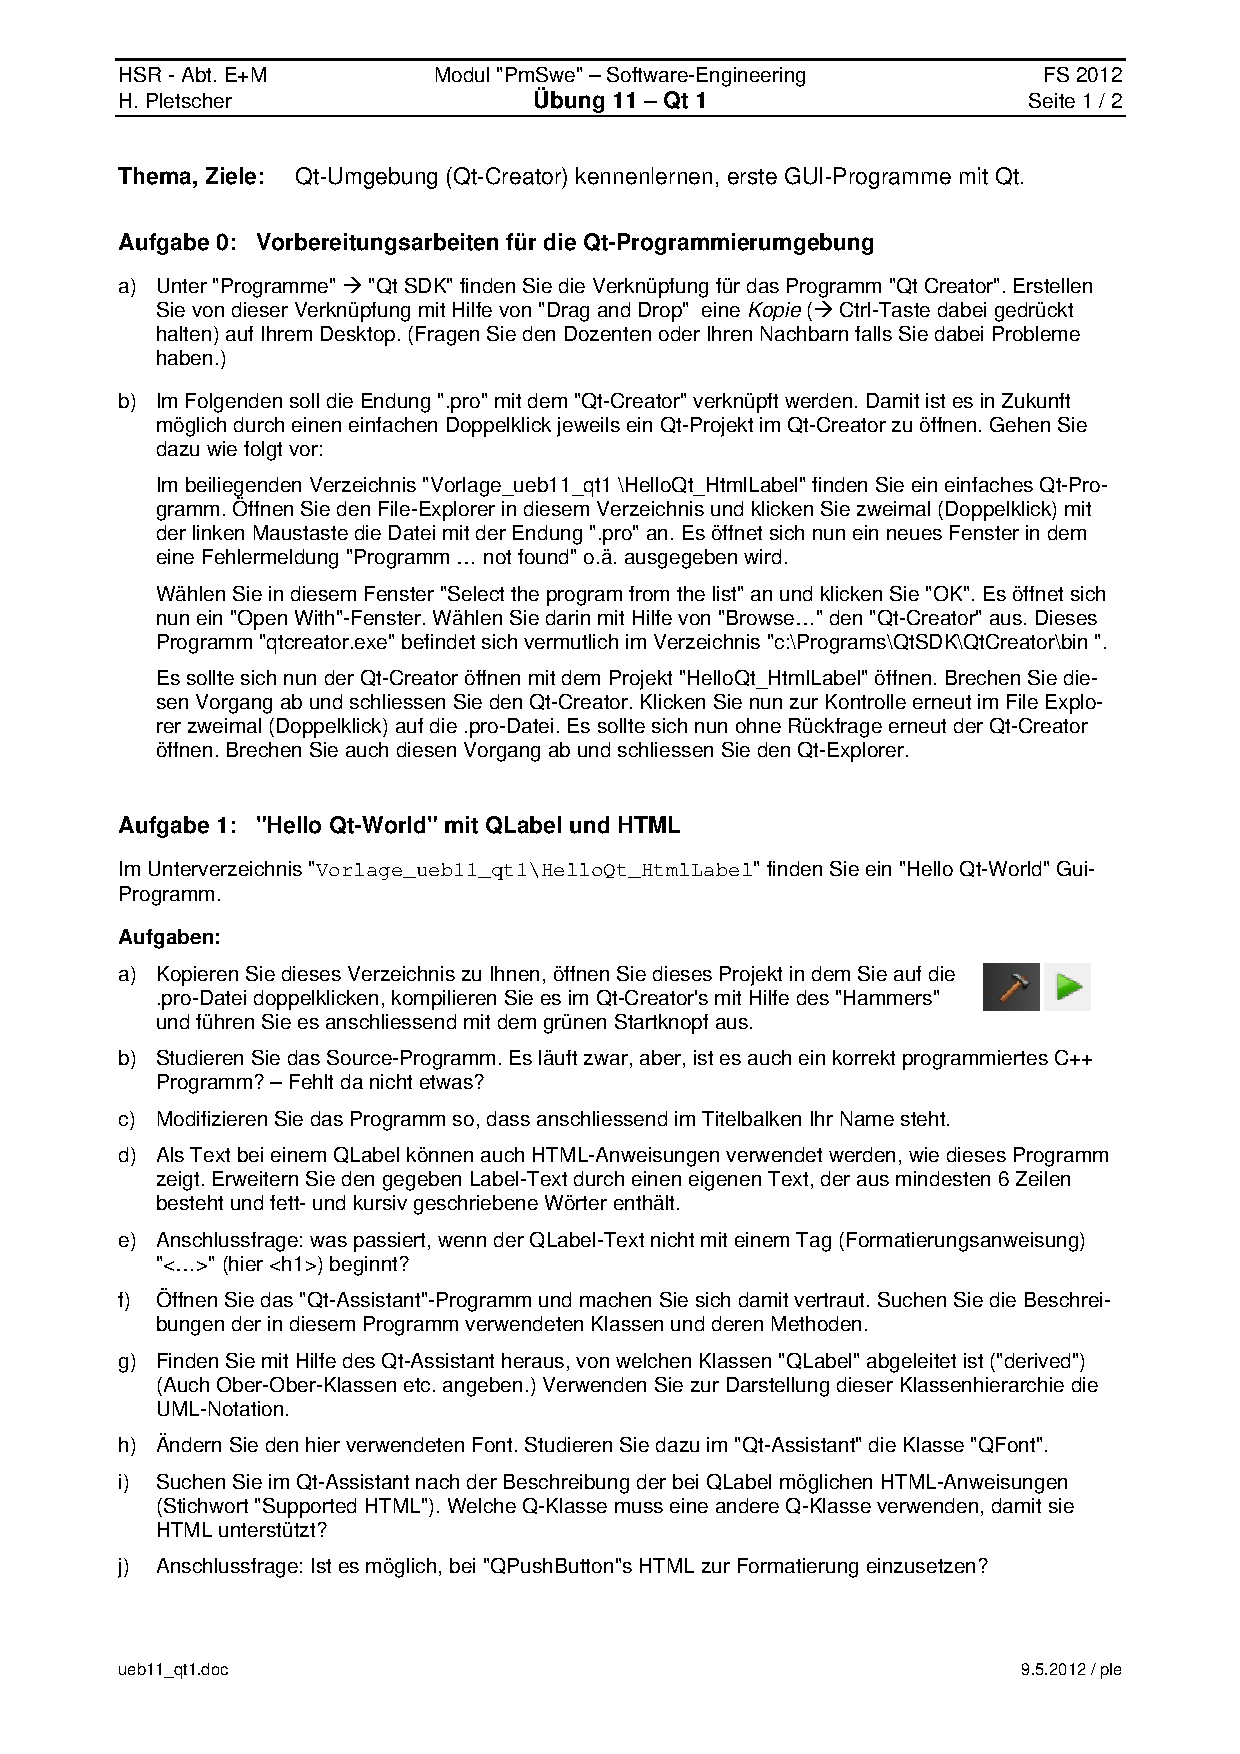
\includepdf[pages=-]{./UebAufgaben/ueb11_qt1.pdf}
\subsection{Lösung Aufgabe 1}
\subsubsection{main.cpp}
\lstinputlisting{./UebLoesungen/LoesUeb11_qt1/lueb11a1_HelloQt_HtmlLabel/main.cpp}
\subsubsection{Qt-Output}
\begin{center}
	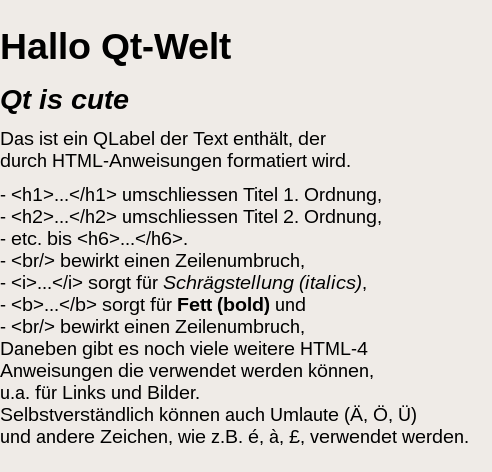
\includegraphics[scale=.5]{./images/u11a1.png}
\end{center}

\subsection{Lösung Aufgabe 2}
\subsubsection{main.cpp}
\lstinputlisting{./UebLoesungen/LoesUeb11_qt1/lueb11a2_HelloQt_PosLabel/main.cpp}
\begin{center}
	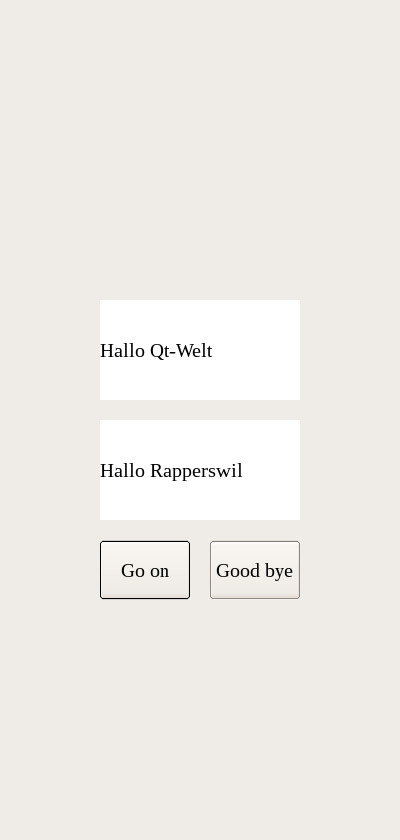
\includegraphics[scale=.5]{./images/u11a2.png}
\end{center}
\subsection{Lösung Aufgabe 3}
\subsubsection{main.cpp}
\lstinputlisting{./UebLoesungen/LoesUeb11_qt1/lueb11a3_HelloQt_Quit/main.cpp}

%Uebung 12
\setcounter{section}{12}
\setcounter{subsection}{1}
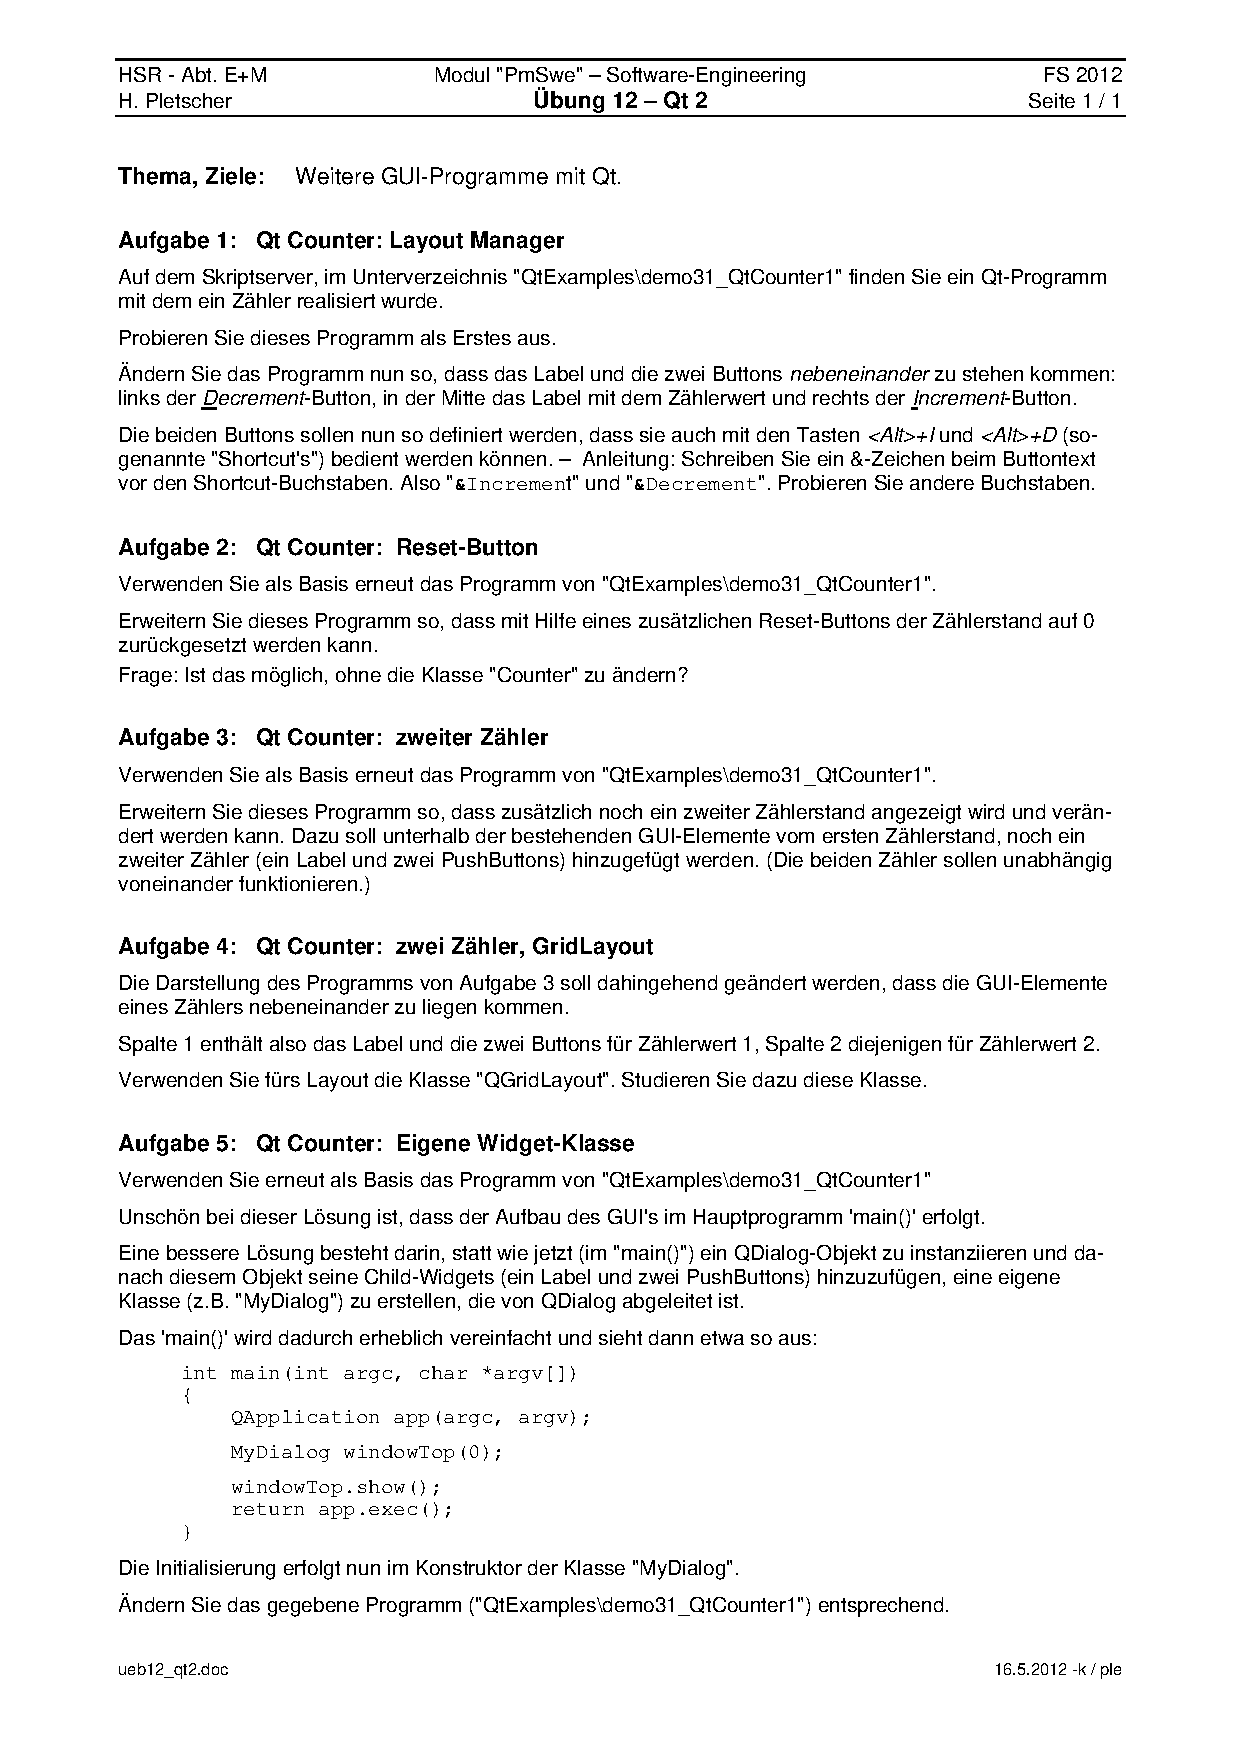
\includepdf[pages=-]{./UebAufgaben/ueb12_qt2.pdf}
\subsection{Lösung}
\subsection{Lösung Aufgabe 1}
\subsubsection{main.cpp}
\lstinputlisting{./UebLoesungen/LoesUeb12_qt2/lueb12a1_CounterLayoutManager/main.cpp}
\subsubsection{counter.cpp}
\lstinputlisting{./UebLoesungen/LoesUeb12_qt2/lueb12a1_CounterLayoutManager/counter.cpp}
\subsubsection{counter.h}
\lstinputlisting{./UebLoesungen/LoesUeb12_qt2/lueb12a1_CounterLayoutManager/counter.h}
\subsubsection{Qt-Output}
\begin{center}
	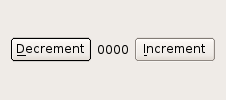
\includegraphics[scale=.5]{./images/u12a1.png}
\end{center}

\subsection{Lösung Aufgabe 2}
\subsubsection{main.cpp}
\lstinputlisting{./UebLoesungen/LoesUeb12_qt2/lueb12a2_CounterResetButton/main.cpp}
\subsubsection{counter.cpp}
\lstinputlisting{./UebLoesungen/LoesUeb12_qt2/lueb12a2_CounterResetButton/counter.cpp}
\subsubsection{counter.h}
\lstinputlisting{./UebLoesungen/LoesUeb12_qt2/lueb12a2_CounterResetButton/counter.h}
\subsubsection{Qt-Output}
\begin{center}
	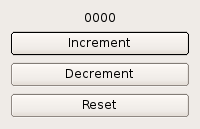
\includegraphics[scale=.5]{./images/u12a2.png}
\end{center}

\subsection{Lösung Aufgabe 3}
\subsubsection{main.cpp}
\lstinputlisting{./UebLoesungen/LoesUeb12_qt2/lueb12a3_CounterZweiZaehler/main.cpp}
\subsubsection{counter.cpp}
\lstinputlisting{./UebLoesungen/LoesUeb12_qt2/lueb12a3_CounterZweiZaehler/counter.cpp}
\subsubsection{counter.h}
\lstinputlisting{./UebLoesungen/LoesUeb12_qt2/lueb12a3_CounterZweiZaehler/counter.h}
\subsubsection{Qt-Output}
\begin{center}
	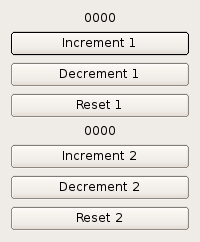
\includegraphics[scale=.5]{./images/u12a3.png}
\end{center}

\subsection{Lösung Aufgabe 4}
\subsubsection{main.cpp}
\lstinputlisting{./UebLoesungen/LoesUeb12_qt2/lueb12a4_CounterGridLayout/main.cpp}
\subsubsection{counter.cpp}
\lstinputlisting{./UebLoesungen/LoesUeb12_qt2/lueb12a4_CounterGridLayout/counter.cpp}
\subsubsection{counter.h}
\lstinputlisting{./UebLoesungen/LoesUeb12_qt2/lueb12a4_CounterGridLayout/counter.h}
\subsubsection{Qt-Output}
\begin{center}
	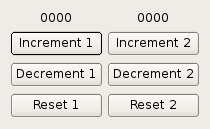
\includegraphics[scale=.5]{./images/u12a4.png}
\end{center}

\subsection{Lösung Aufgabe 5}
\subsubsection{main.cpp}
\lstinputlisting{./UebLoesungen/LoesUeb12_qt2/lueb12a5_CounterWidget/main.cpp}
\subsubsection{Counter.cpp}
\lstinputlisting{./UebLoesungen/LoesUeb12_qt2/lueb12a5_CounterWidget/Counter.cpp}
\subsubsection{Counter.h}
\lstinputlisting{./UebLoesungen/LoesUeb12_qt2/lueb12a5_CounterWidget/Counter.h}
\subsubsection{MyDialog.cpp}
\lstinputlisting{./UebLoesungen/LoesUeb12_qt2/lueb12a5_CounterWidget/MyDialog.cpp}
\subsubsection{MyDialog.h}
\lstinputlisting{./UebLoesungen/LoesUeb12_qt2/lueb12a5_CounterWidget/MyDialog.h}
\subsubsection{Qt-Output}
\begin{center}
	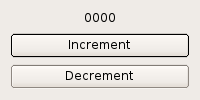
\includegraphics[scale=.5]{./images/u12a5.png}
\end{center}

%Uebung 13
\setcounter{section}{13}
\setcounter{subsection}{1}
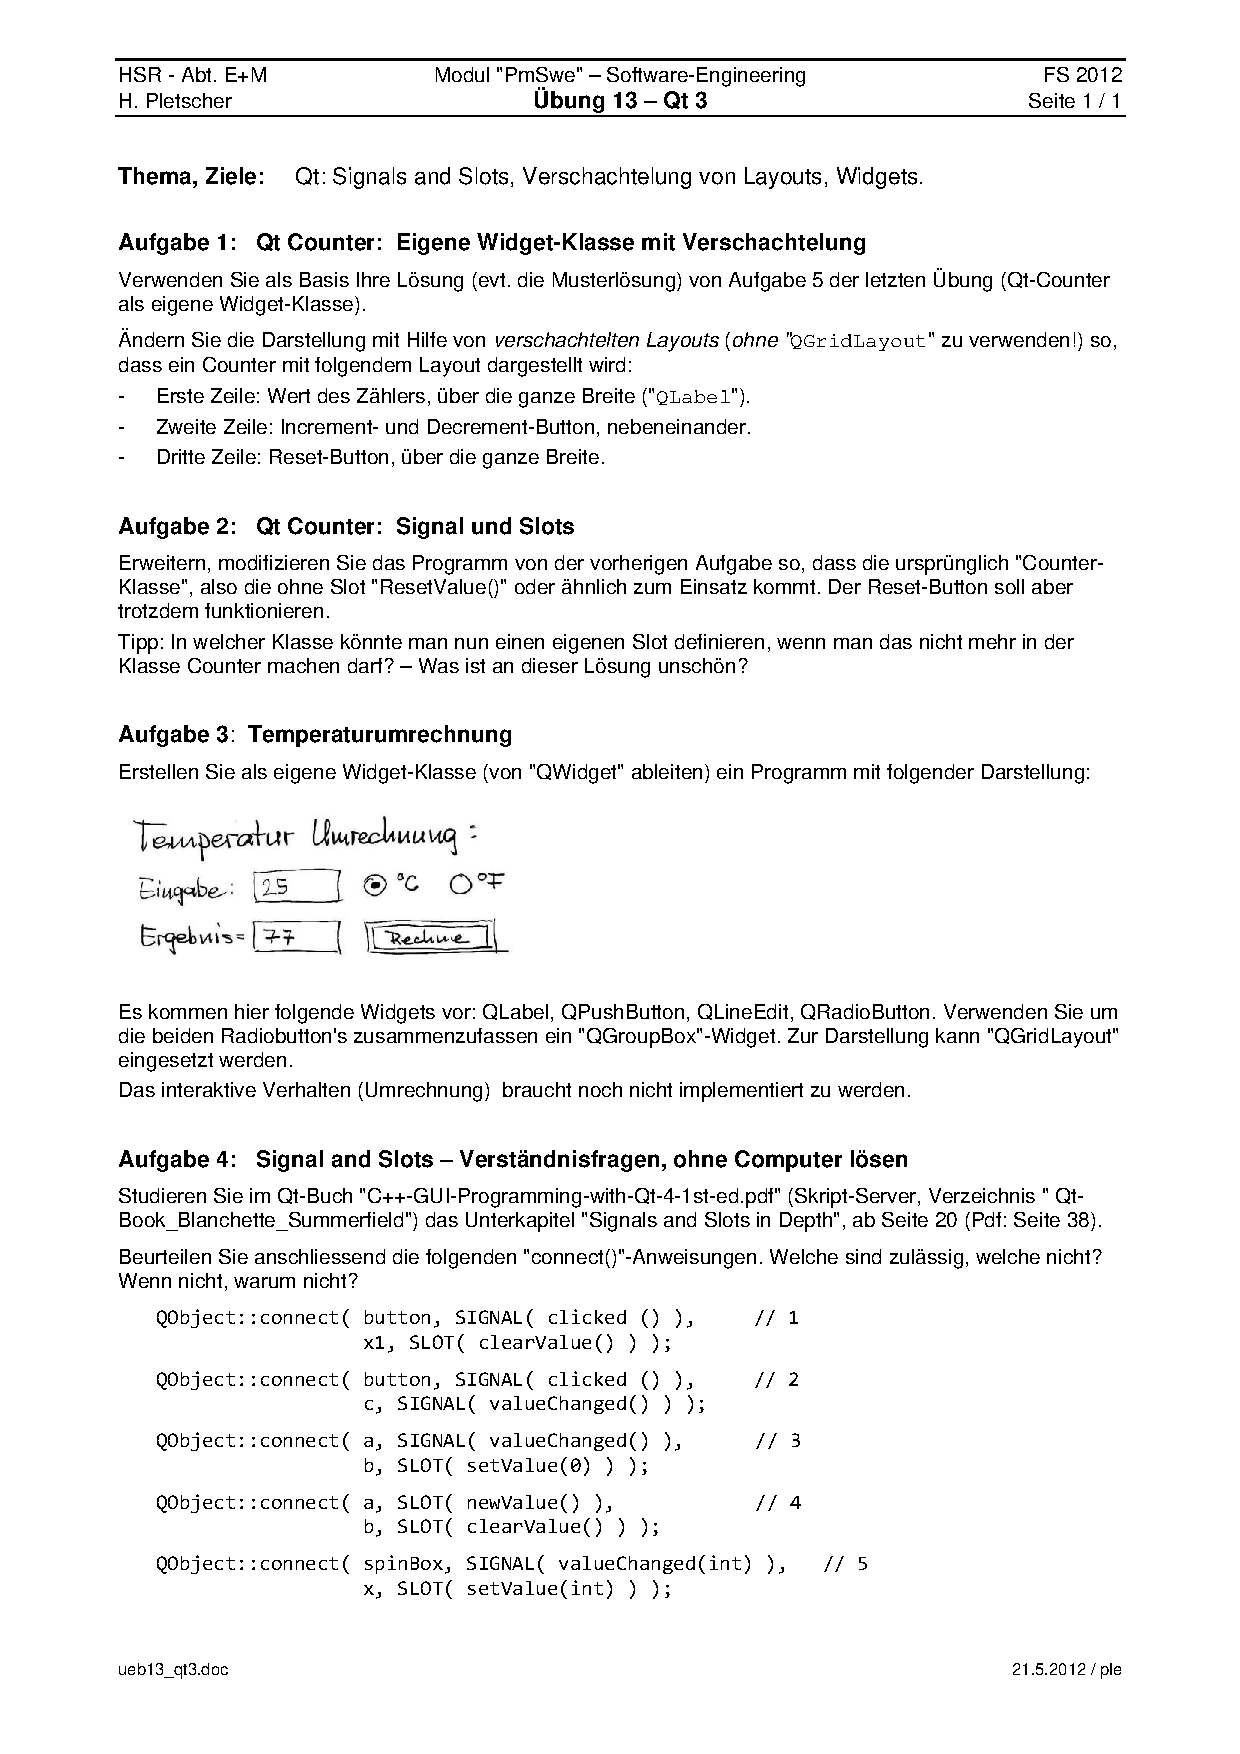
\includepdf[pages=-]{./UebAufgaben/ueb13_qt3.pdf}
\subsection{Lösung Aufgabe 1}
\subsubsection{main.cpp}
\lstinputlisting{./UebLoesungen/LoesUeb13_qt3/lueb13a1_CounterWidgetNested/main.cpp}
\subsubsection{Counter.cpp}
\lstinputlisting{./UebLoesungen/LoesUeb13_qt3/lueb13a1_CounterWidgetNested/Counter.cpp}
\subsubsection{Counter.h}
\lstinputlisting{./UebLoesungen/LoesUeb13_qt3/lueb13a1_CounterWidgetNested/Counter.h}
\subsubsection{MyDialog.cpp}
\lstinputlisting{./UebLoesungen/LoesUeb13_qt3/lueb13a1_CounterWidgetNested/MyDialog.cpp}
\subsubsection{MyDialog.h}
\lstinputlisting{./UebLoesungen/LoesUeb13_qt3/lueb13a1_CounterWidgetNested/MyDialog.h}
\subsubsection{Qt-Output}
\begin{center}
	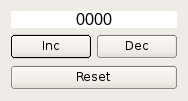
\includegraphics[scale=.5]{./images/u13a1.png}
\end{center}

\subsection{Lösung Aufgabe 2}
\subsubsection{main.cpp}
\lstinputlisting{./UebLoesungen/LoesUeb13_qt3/lueb13a2_CounterOwnSlot/main.cpp}
\subsubsection{Counter.cpp}
\lstinputlisting{./UebLoesungen/LoesUeb13_qt3/lueb13a2_CounterOwnSlot/Counter.cpp}
\subsubsection{Counter.h}
\lstinputlisting{./UebLoesungen/LoesUeb13_qt3/lueb13a2_CounterOwnSlot/Counter.h}
\subsubsection{MyDialog.cpp}
\lstinputlisting{./UebLoesungen/LoesUeb13_qt3/lueb13a2_CounterOwnSlot/MyDialog.cpp}
\subsubsection{MyDialog.h}
\lstinputlisting{./UebLoesungen/LoesUeb13_qt3/lueb13a2_CounterOwnSlot/MyDialog.h}

\subsection{Lösung Aufgabe 3}
\subsubsection{main.cpp}
\lstinputlisting{./UebLoesungen/LoesUeb13_qt3/lueb13a3_TempWidgetView/main.cpp}
\subsubsection{TemperaturWidget.cpp}
\lstinputlisting{./UebLoesungen/LoesUeb13_qt3/lueb13a3_TempWidgetView/TemperaturWidget.cpp}
\subsubsection{TemperaturWidget.h}
\lstinputlisting{./UebLoesungen/LoesUeb13_qt3/lueb13a3_TempWidgetView/TemperaturWidget.h}
\subsubsection{Qt-Output}
\begin{center}
	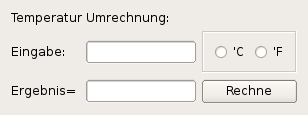
\includegraphics[scale=.5]{./images/u13a3.png}
\end{center}

\subsection{Lösung Aufgabe 4}
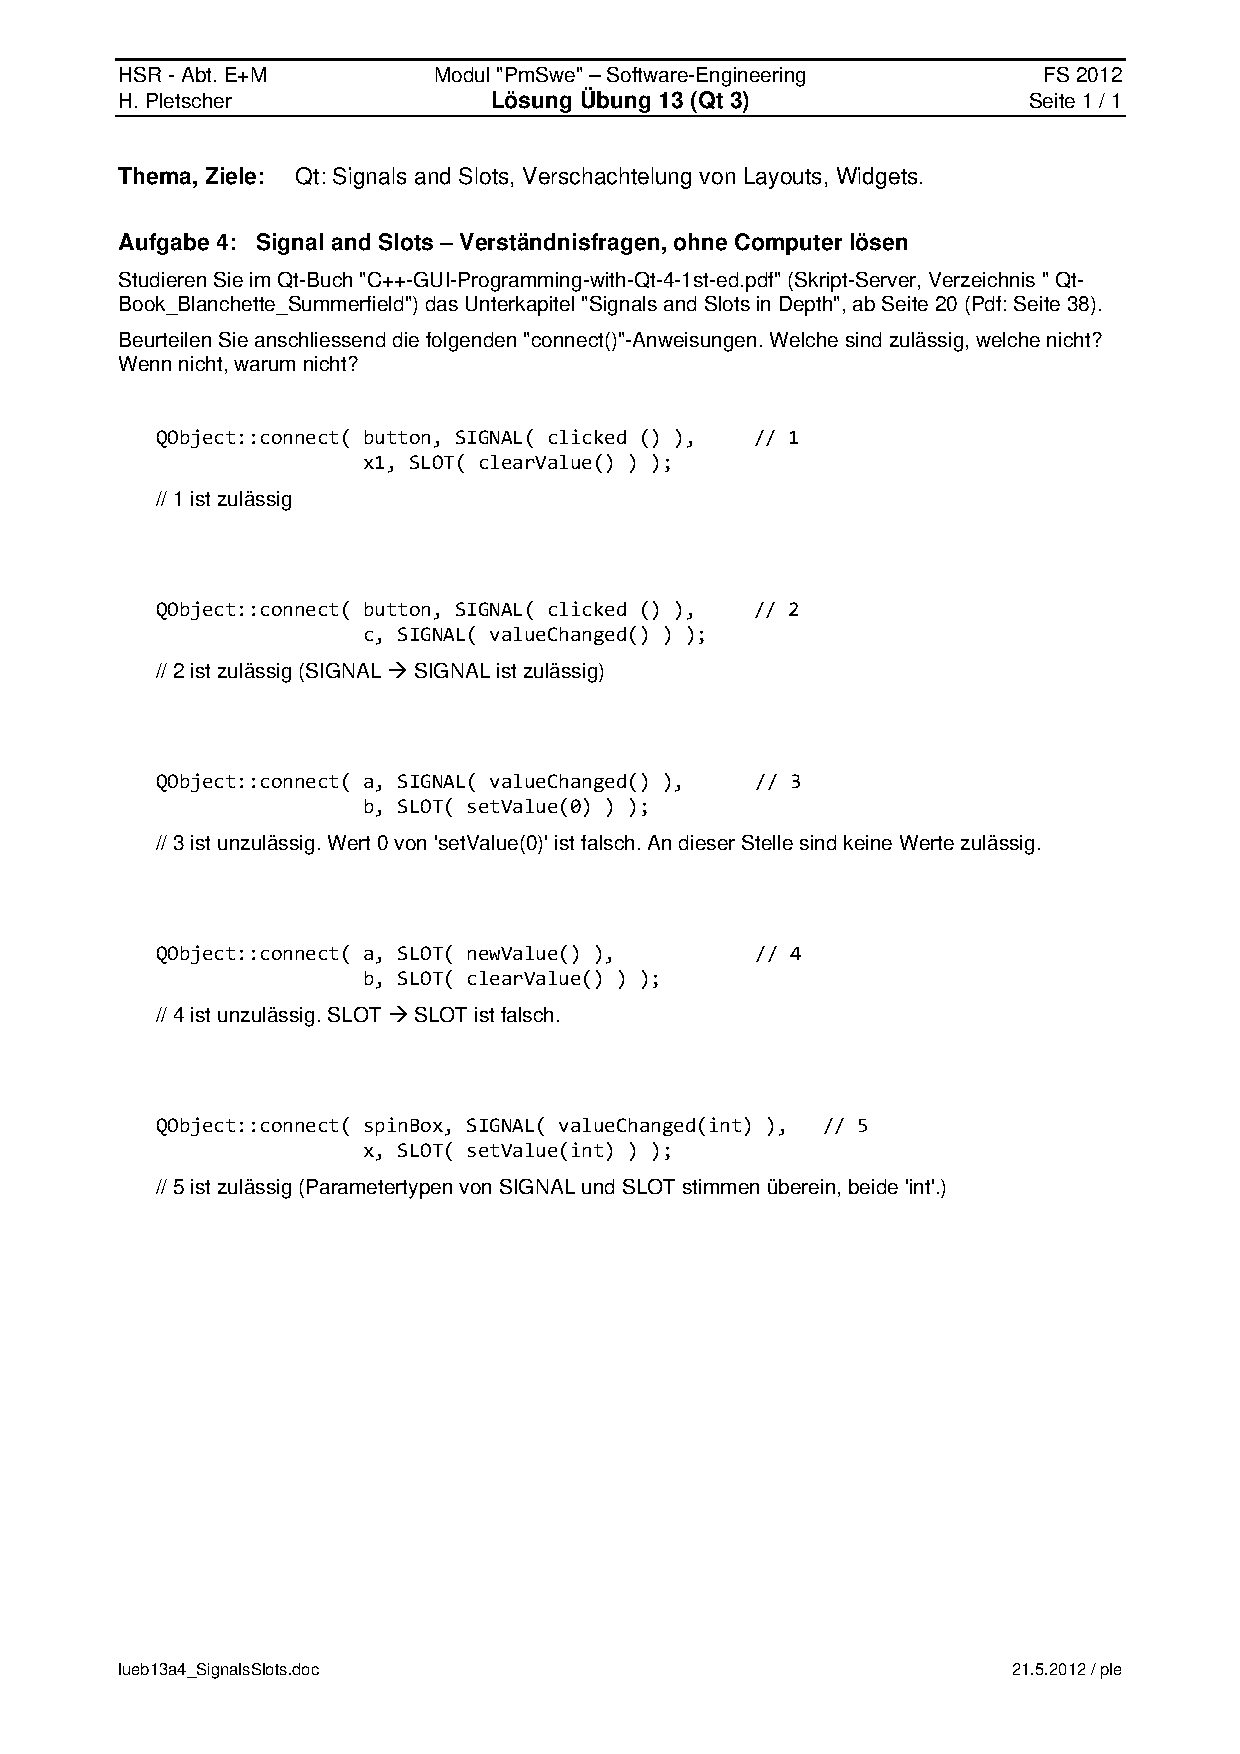
\includepdf[pages=-]{./UebLoesungen/LoesUeb13_qt3/lueb13a4_SignalsSlots.pdf}

%Uebung 14
\setcounter{section}{14}
\setcounter{subsection}{1}
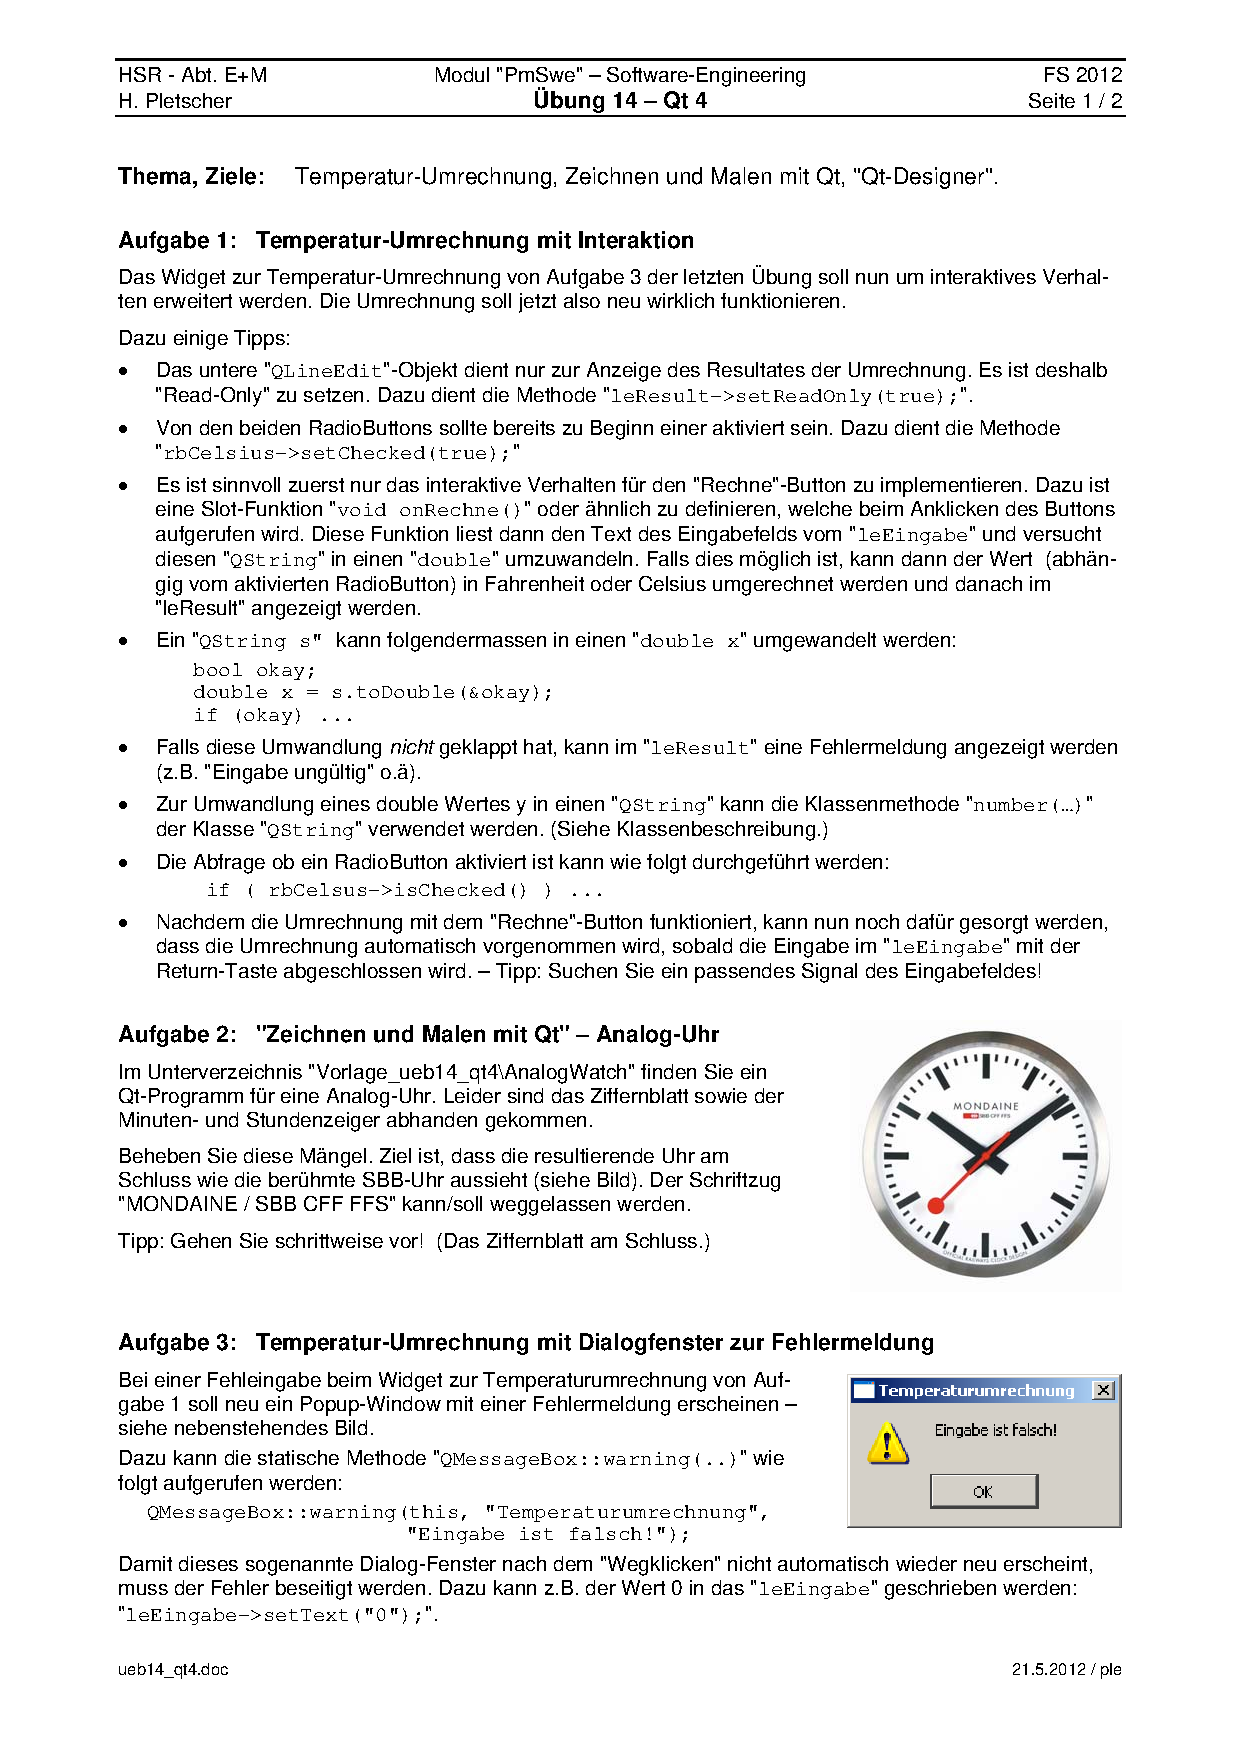
\includepdf[pages=-]{./UebAufgaben/ueb14_qt4.pdf}
\subsection{Lösung Aufgabe 1}
\subsubsection{main.cpp}
\lstinputlisting{./UebLoesungen/LoesUeb14_qt4/lueb14a1_TempWidget/main.cpp}
\subsubsection{TemperaturWidget.cpp}
\lstinputlisting{./UebLoesungen/LoesUeb14_qt4/lueb14a1_TempWidget/TemperaturWidget.cpp}
\subsubsection{TemperaturWidget.h}
\lstinputlisting{./UebLoesungen/LoesUeb14_qt4/lueb14a1_TempWidget/TemperaturWidget.h}
\subsubsection{Qt-Output}
\begin{center}
	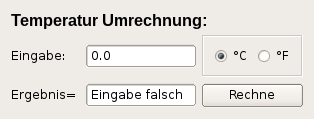
\includegraphics[scale=.5]{./images/u14a1.png}
\end{center}

\subsection{Lösung Aufgabe 2}
\subsubsection{main.cpp}
\lstinputlisting{./UebLoesungen/LoesUeb14_qt4/lueb14a2_AnalogWatch/main.cpp}
\subsubsection{AnalogWatch.cpp}
\lstinputlisting{./UebLoesungen/LoesUeb14_qt4/lueb14a2_AnalogWatch/AnalogWatch.cpp}
\subsubsection{AnalogWatch.h}
\lstinputlisting{./UebLoesungen/LoesUeb14_qt4/lueb14a2_AnalogWatch/AnalogWatch.h}
\subsubsection{Qt-Output}
\begin{center}
	
\includegraphics[scale=.5]{./images/u14a2.png}
\end{center}

\subsection{Lösung Aufgabe 3}
\subsubsection{main.cpp}
\lstinputlisting{./UebLoesungen/LoesUeb14_qt4/lueb14a3_TempWidgetWithDialog/main.cpp}
\subsubsection{TemperaturWidget.cpp}
\lstinputlisting{./UebLoesungen/LoesUeb14_qt4/lueb14a3_TempWidgetWithDialog/TemperaturWidget.cpp}
\subsubsection{TemperaturWidget.h}
\lstinputlisting{./UebLoesungen/LoesUeb14_qt4/lueb14a3_TempWidgetWithDialog/TemperaturWidget.h}


TODO: Ein Hirsch mit installiertem kiuuut soll doch alle skriinschöts machen

